\section{Yield extraction}

Extended unbinned maximum likelihood fits are used to extract the yields of the rare and resonant channels.
The likelihood has the form:
%
\begin{equation}
\mathcal{L}=e^{-(N_\mathrm{S}+N_\mathrm{C}+N_{\mathrm{B}})}\times\prod_{i=1}^{N}\left[
N_\mathrm{S}P_{\mathrm{S}}(m_i)+N_\mathrm{C}P_\mathrm{C}(m_i)+N_{\mathrm{B}}P_{\mathrm{B}}(m_i)\right]
\end{equation}
\noindent
where $N_\mathrm{S}$, $N_\mathrm{C}$ and $N_\mathrm{B}$ are respectively the numbers of signal, 
combinatorial and \KS background events and the $P_i(m_i)$ are the corresponding probability density functions (PDF).
The fit variable is the 4-body $m(p\pi\mu\mu)$ invariant mass obtained from
a kinematical fit of the full decay chain in which each particle is constrained to point to its
assigned origin vertex and the invariant mass of the $p\pi$ system is constrained to be equal to
the world average for the \Lz baryon mass. In the resonant case a further constrain is used on the dimuon
mass to be equal to the known \jpsi mass. This method allows to improve the mass resolution giving
better defined peaks and therefore a more stable fit. For brevity, in the following these variables are
simply referred to as ``invariant mass".

\subsection{Fit description}
\label{sec:Lb_fit}

The fit is performed though the following steps:
%
\begin{itemize}
\item simulated distributions are fit to extract initial parameters;
\item the resonant data sample is fitted;
\item the rare sample is fitted fixing some parameters to those obtained in the previous cases.
\end{itemize}
%

In the first step simulated $\Lb\to\jpsi\Lz$ distributions are fitted using the signal PDF alone.
This is done separately for long and downstream candidates. Figure~\ref{fig:Lb_jpsiMCfit} shows 
distributions of candidates selected in the resonant sample with the fit function overlaid.
%
The signal is described as the sum of two Crystal Ball functions (CB) with
common mean ($m_0$) and tail slope ($n$). This is also known as Double Crystal Ball (DCB) function.
A single Crystal Ball~\cite{Skwarnicki:1986xj} is a probability
density function commonly used to model processes involving energy loss. In particular it is used
to describe resonances' peaks with radiative tails. This function 
consists of a Gaussian core and a power-law tail below a certain threshold and has form
%
\begin{equation}
C(x;\alpha,n,\bar{x},\sigma) = N \cdot
\begin{cases}
exp \left( -\frac{(x - \bar{x})^2}{2\sigma} \right)  & \mbox{   if   } \frac{(x - \bar{x})}{\sigma} > \alpha, \\
A\left( B - \frac{(x - \bar{x})}{\sigma} \right)^{-n} & \mbox{   if   } \frac{(x - \bar{x})}{\sigma} < \alpha,
\end{cases}
\end{equation}
%
where for normalisation and continuity
%
\begin{equation}
\label{CB}
\begin{array}{ll}
A = \left( \frac{c}{|\alpha|} \right))^n \cdot exp(- \frac{\alpha^2}{2}), \\
B = \frac{n}{|\alpha|} - |\alpha|.
\end{array}
\end{equation}
%
The full PDF for the resonant channel is therefore:
%
\begin{equation}
P_\mathrm{S}(m;m_0,\alpha_1,\alpha_2,f,n) = f \text{CB}(m;m_0,\sigma_1,\alpha_1,n)+(1-f)\text{CB}(m;m_0,\sigma_2,\alpha_2,n),
\end{equation}
%
where $f$ is the relative fraction of candidates falling into the first CB function.

\begin{figure}
\centering
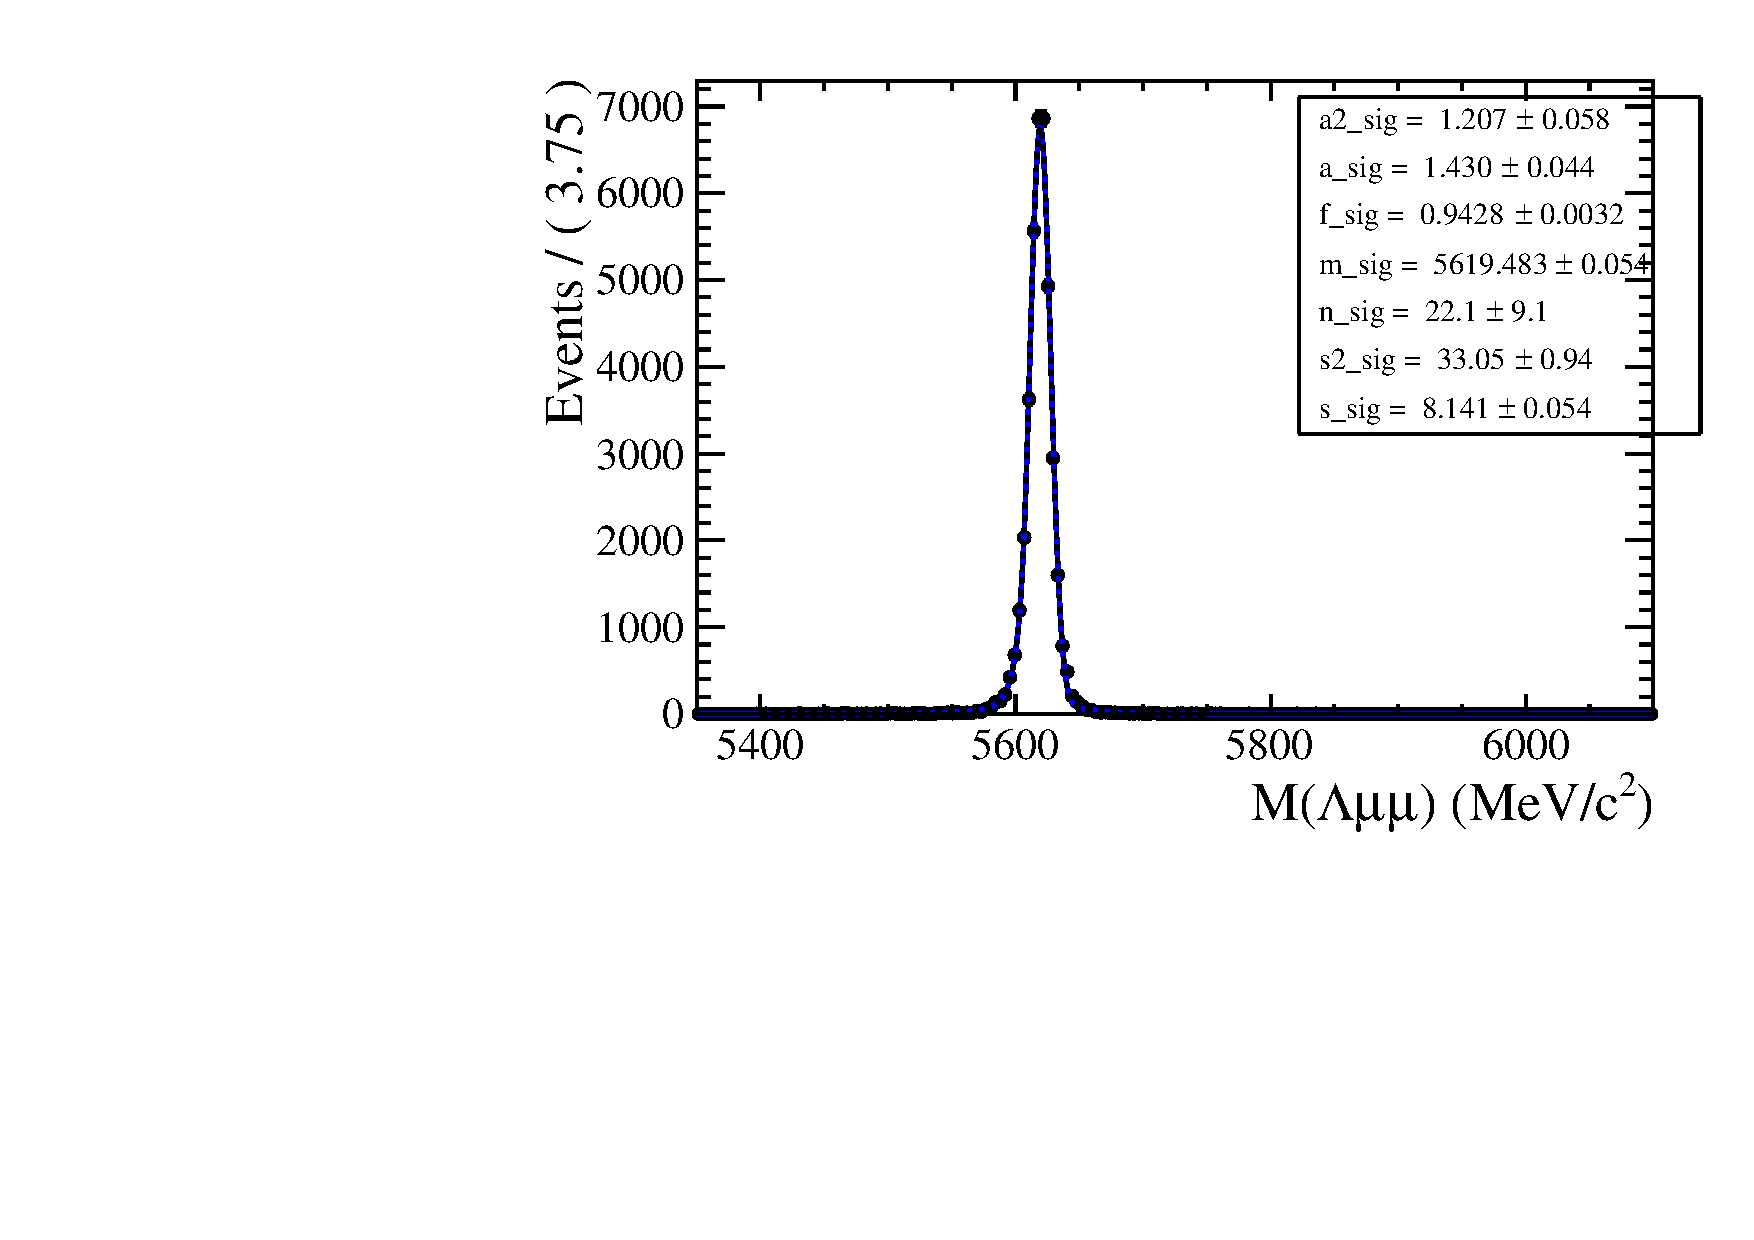
\includegraphics[width=0.49\textwidth]{Lmumu/figs/MassFits/fitLb2JpsiL_DD_MC.pdf}
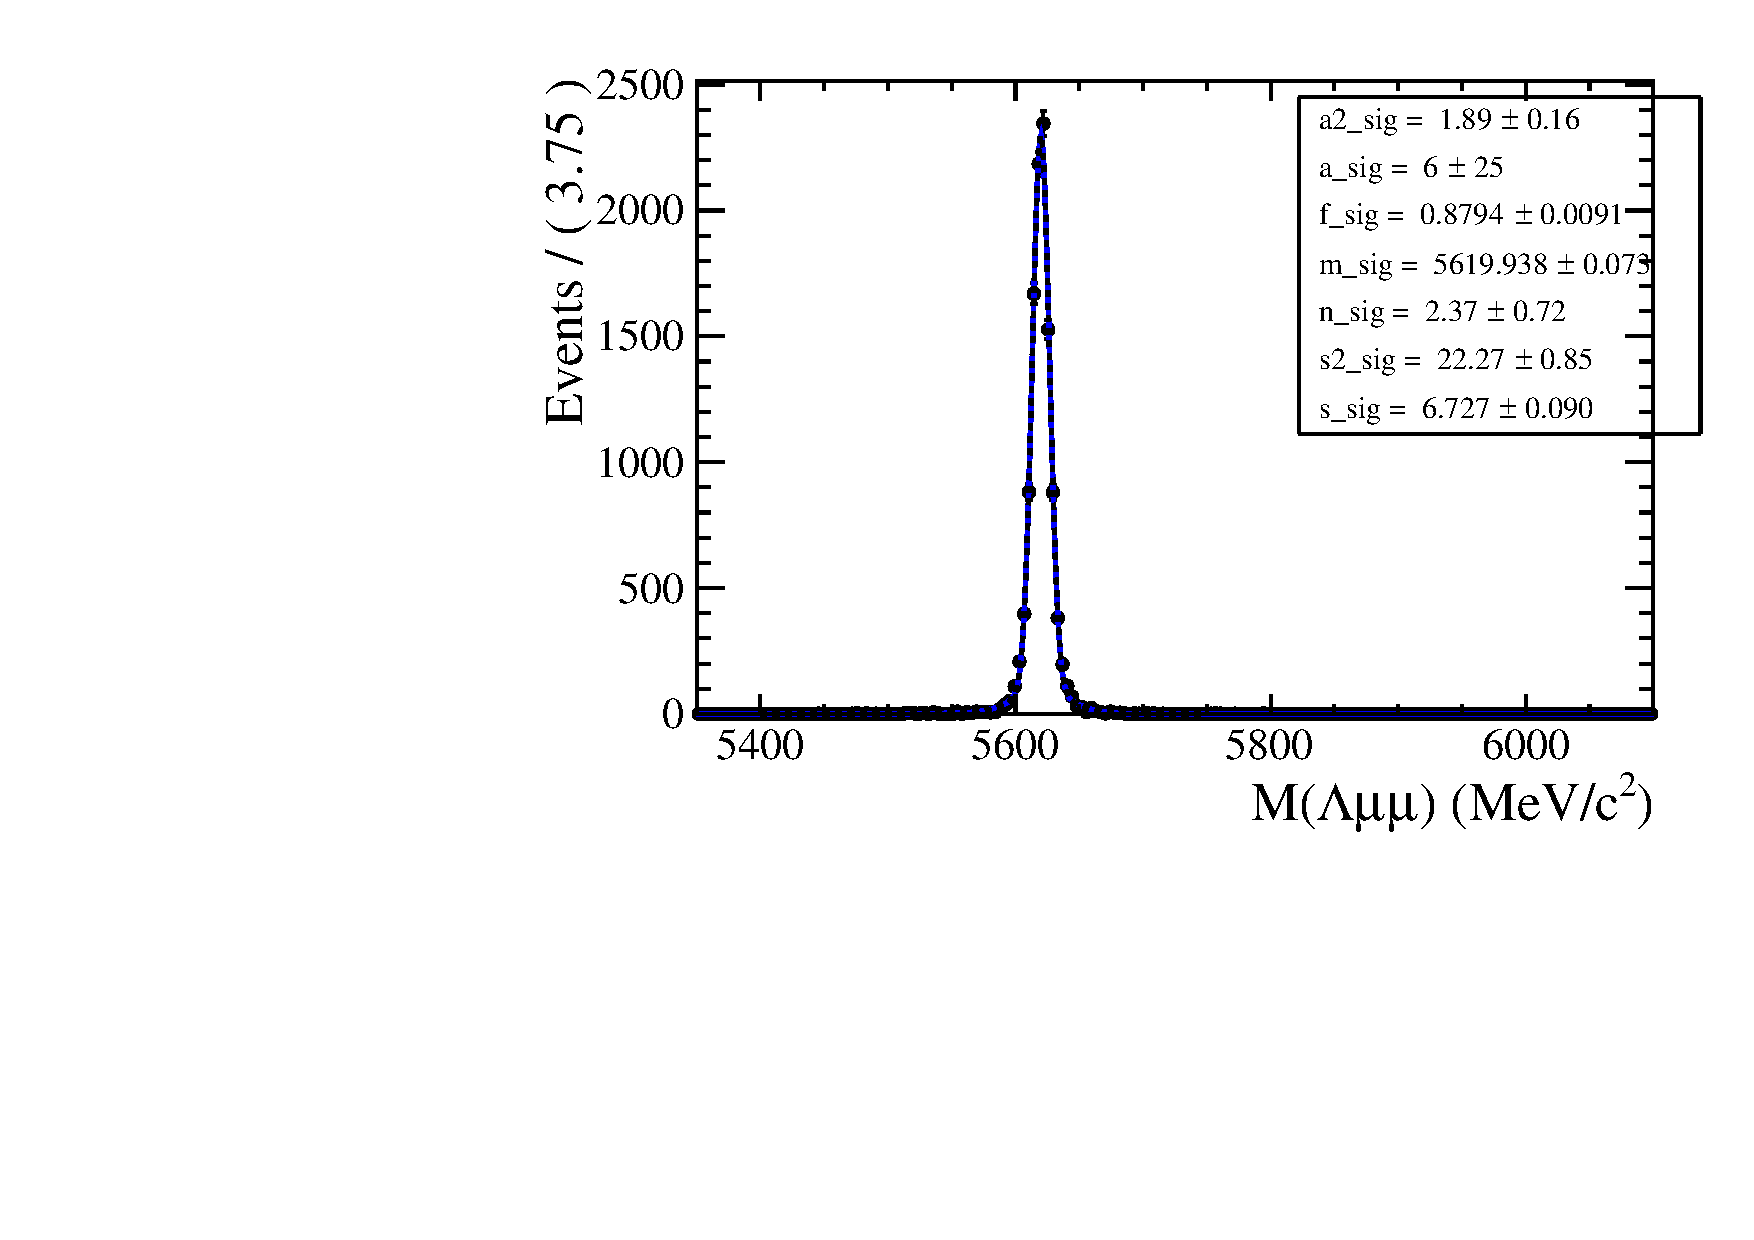
\includegraphics[width=0.49\textwidth]{Lmumu/figs/MassFits/fitLb2JpsiL_LL_MC.pdf}
\caption{Invariant mass distribution of $\Lb\ra\Lz\jpsi$ downstream (left) long (right) candidates.
The points show simulated data and the blue line is the signal fit function.}
\label{fig:Lb_jpsiMCfit}
\end{figure}

In a second step the fit to the resonant channel data sample is performed.
For this fit the tail slope parameter, ``$n$", which is highly correlated
with $\alpha_1$ and $\alpha_2$, is fixed to the value found in the fit to simulated data.
In this fit two background components are modelled: the combinatorial background,
parameterized with an exponential and the background from $\Bz\ra\jpsi\KS$ decays.
The shape used to describe the \KS background is obtained from a $\Bz\ra\jpsi\KS$ simulated
sample to which the full selection is applied. The invariant distribution of these events
is fit with a DCB function, which is then used to model the \KS background
in the $\Lb\to\jpsi\Lz$ fit. The fit to the simulated $\Bz\ra\jpsi\KS$ events
is reported in Fig.~\ref{fig:KSbkgFit}. When the \KS shape is introduced in the fit to the data all
its parameters are fixed. This is particularly important when fitting long candidates, where the \KS
peak is less evident, which does not allow to constrain many parameters. On the other hand, in order
to take into account possible data-simulation differences, an horizontal shift is added and left
floating (by adding a constant to the central value of the DCB, $m_0 \ra m_0 + m'$).
In summary, the free parameters in the fit to the resonant $\Lb\to\jpsi\Lz$ sample
are the yields of the signal and the combinatorial and \KS backgrounds, the slope
of the exponential and the horizontal shift of the \KS shape. Note that all parameters
of the fit to the long and downstream samples are independent.

\begin{figure}
\centering
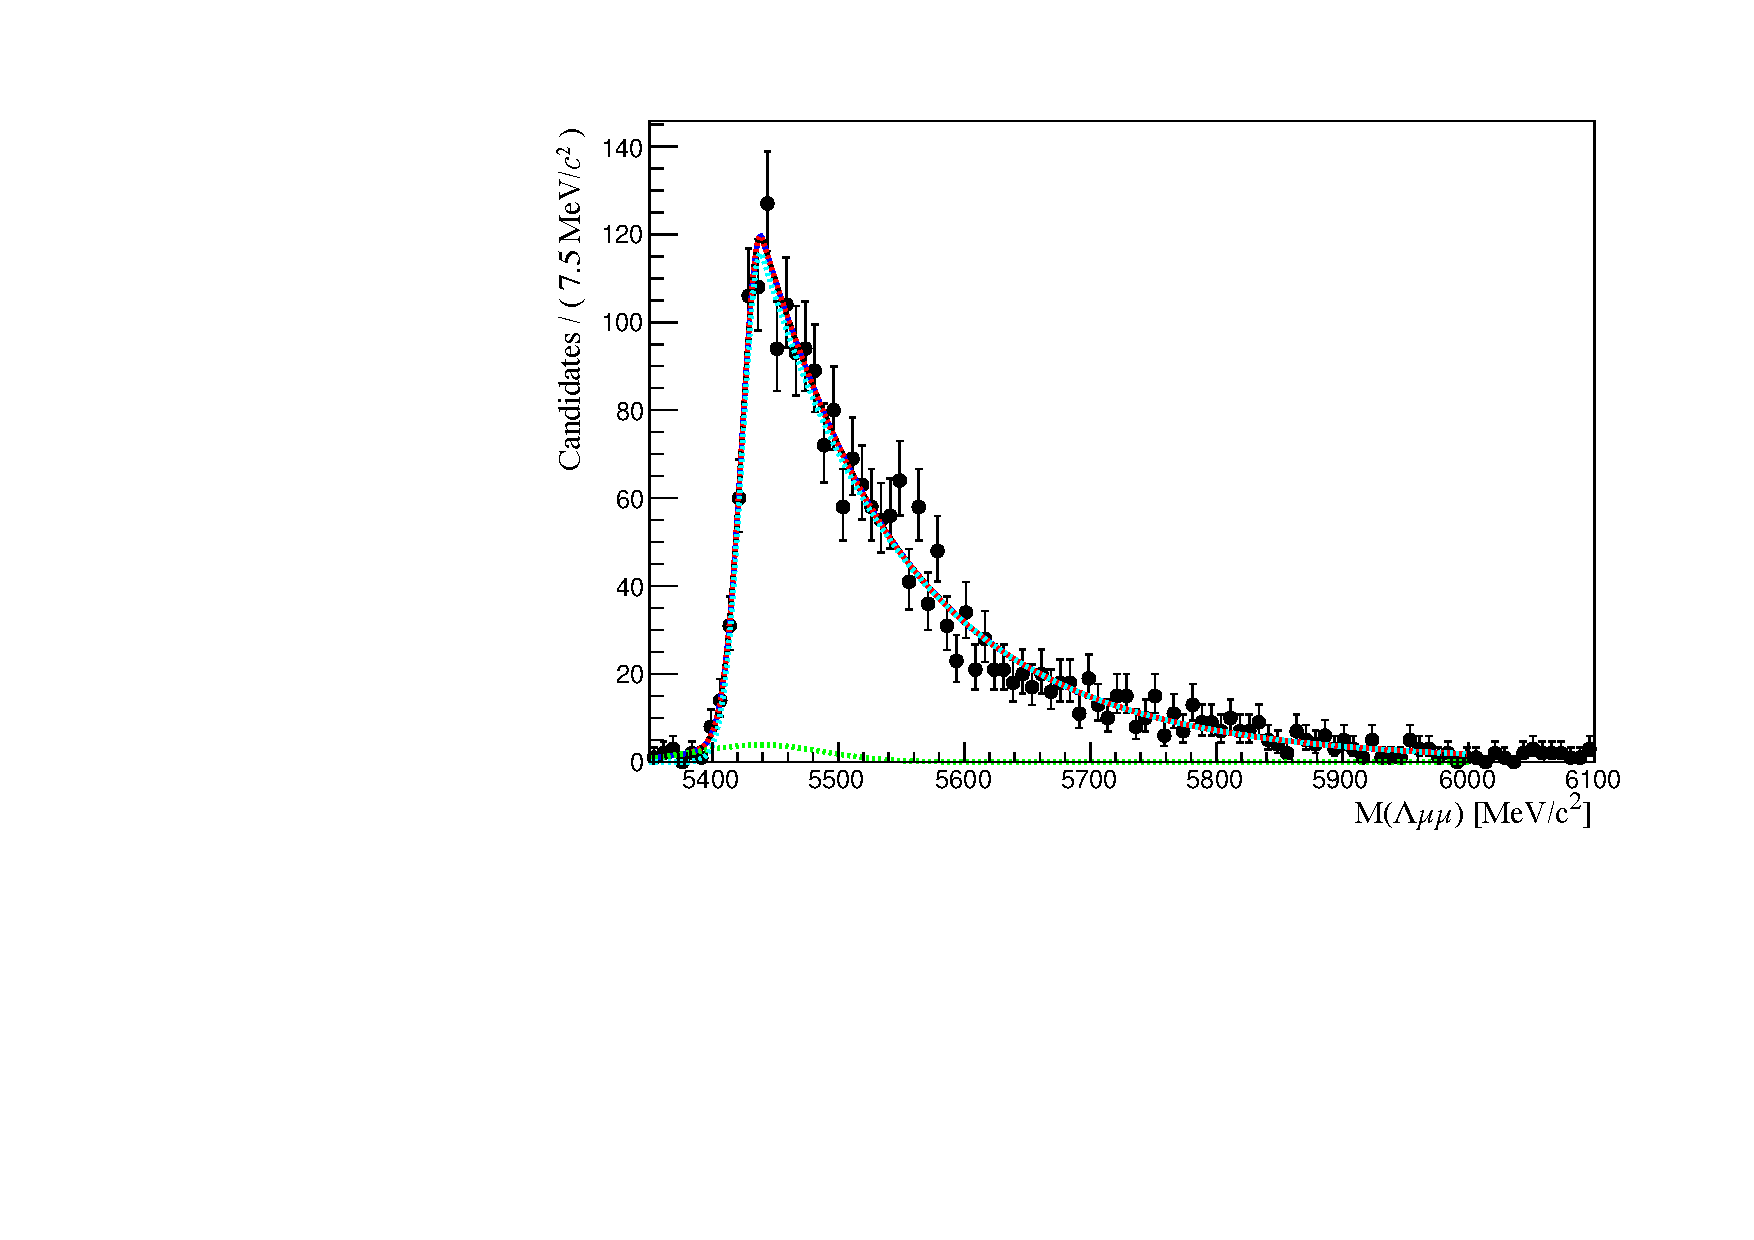
\includegraphics[width=0.6\textwidth]{Lmumu/figs/MassFits/fitKS_bkg.pdf}
\caption{Invariant mass distribution of simulated $\Bz\ra\jpsi\KS$ events after 
full selection fitted a Double Crystal Ball function. }
\label{fig:KSbkgFit}
\end{figure}

Finally, the rare $\Lb\to\Lz\mumu$ data sample is fit. In this case the fit to the long
and downstream samples is performed simultaneously to obtain a more stable convergence. 
In this fit the signal is modelled with the same shape used in the resonant case as there is no physical
reason why they should be different. This method is also useful to limit systematic uncertainties
as the result will be given as a ratio between rare and resonant quantities.
However, the low statistics for the rare sample does not allow to constrain many parameters.
%,especially when dividing data in \qsq bins.
Therefore, all parameters of the signal shape are fixed to
the ones derived from the fit to the normalisation channel. However, to account for possible differences, 
arising from a different resolution in different \qsq regions, a scale factor is multiplied
to the widths of the two gaussian cores of the signal DCB: $\sigma_1 \rightarrow c\cdot \sigma_1$
and $\sigma_2 \rightarrow c\cdot \sigma_2$, where the two scale factors are the same. This factors
are fixed in the fit to data by fitting rare $\Lb\to\Lz\mumu$ simulated events in each \qsq bin and comparing
the widths with the ones found on the fit to the resonant simulated sample, namely
\begin{equation}
c = \sigma_{\mumu}^{MC} / \sigma_{\jpsi}^{MC}.
\end{equation}
Values obtained are $\sim 1.9$ for downstream candidates and $\sim 2.3$ for long candidates,
corresponding to the fact that in the resonant case a further constrain on the dimuon mass
is used, which improves the resolution by a factor of $\sim2$. The dependence of the scaling factor on \qsq 
is found to be small. For the fits on the long and downstream samples the parameters are always fixed to the
corresponding \jpsi fit; in this analysis shape parameters are never shared between the two candidate categories.

Also in the rare case the modelled background components are
the combinatorial background, described with an exponential function and the \KS background. 
The slope of the background is visibly different depending on the \qsq interval. This is partly due to the 
fact that at high \qsq the combinatorial changes slope because of a kinematical limit at low 4-body
masses imposed by the \qsq requirements. The exponential slopes are therefore left as independent
parameters in each \qsq interval. % and for the downstream and long samples.
The background component from $\Bz\to\KS\mumu$ decays is modelled using the same shapes used
for the resonant channel. However, in this case the horizontal shift is fixed to what found
for the resonant channel. The expected amount of misreconstructed $\Bz\ra\KS\mumu$
events is small and does not allow to determine reliably the yield. Therefore
this is fixed to the yield of $\Bz\ra\jpsi\KS$ decays rescaled by the expected ratio
of branching fractions between the resonant and rare channels. The \qsq distribution of $\Bz\ra\KS\mumu$ 
simulated events is used to predict the yield as a function of \qsq. Table~\ref{tab:KSprediction} reports the 
number of predicted $\Bz\ra\KS\mumu$ events in each \qsq interval obtained with the following formula:
\begin{equation}
N_{\KS\mumu}(\qsq) = N_{\jpsi\KS}\frac{B(\Bz\ra\KS\mumu)}{B(\Bz\ra\KS\jpsi)}\cdot \frac{1}{\epsilon_{rel}} \cdot B(\jpsi\ra\mumu) \frac{N(\qsq)_{MC}}{N^{tot}_{MC}} 
\end{equation}
where $N(\qsq)_{MC}$ is the number of simulated rare candidates falling in a \qsq interval after full selection and $N^{tot}_{MC}$ 
is the total number of simulated events. 
%The \KS\mumu contribution is then completely taken out to study systematic
%uncertainties as described in Sec.~\ref{sec:Lb_sys}.
%Only for the 6-8 \gevgevcccc bin, a background component coming from the residual of the \jpsi radiative tail is
%added, modelled using a the shape obtained studying simulated events and smoothed using the \verb!RooKeysPdf! method of \verb!RooFit!.
%This is then removed from the final fit becuase it returns zero yield.

\begin{table}
\centering
\caption{Predicted numbers of $\Bz\ra\KS\mumu$ events in each considered \qsq interval.}
\begin{tabular}{$l^c^c}
	\rowstyle{\bfseries}
 \qsq interval [\gevgevcccc]  & Downstream & Long \\ \hline
0.1--2.0 & 0.9 & 0.1 \\
2.0--4.0 & 0.9 & 0.1 \\
4.0--6.0 & 0.8 & 0.1 \\
6.0--8.0 & 1.1 & 0.1 \\
11.0--12.5 & 1.9 & 0.2 \\
15.0--16.0 & 1.1 & 0.1 \\
16.0--18.0 & 2.0 & 0.2 \\
18.0--20.0 & 1.1 & 0.1 \\ \hline
1.1--6.0 & 2.1 & 0.1 \\
15.0--20.0 & 4.2 & 0.5 \\ 
\end{tabular}
\label{tab:KSprediction}
\end{table}

As the fit on the rare sample is performed simultaneously on long and downstream candidates,
their two yields are not free to vary separately but are parameterised
as a function of the common branching fraction using the following formula:
%
\begin{equation}
N(\Lz\mumu)_{k}  = \left[ \frac{\mathrm{d}\mathcal{B}(\Lz\mumu)/\mathrm{d}\qsq}{\mathcal{B}(\jpsi\Lz)} \right]  \cdot
N(\jpsi\Lz)_{k} \cdot \varepsilon^{\mathrm{rel}}_{k} \cdot \frac {\Delta\qsq} { \mathcal{B}(\jpsi\to\mumu) },
\label{eq:relYield}
\end{equation}
%
where $k = $(LL,DD), $\Delta\qsq$ is the width of the \qsq interval and the only free parameter is the relative branching 
fraction ratio of the rare over \jpsi channels. For the branching fraction of the \jpsi\to\mumu decay the value 
reported in the PDG book, \mbox{$(5.93 \pm 0.06)\cdot 10^{-2}$~\cite{PDG2014}} is used and $\varepsilon^{rel}$ corresponds to
the relative efficiency between the rare and resonant channels obtained in Sec.~\ref{sec:Lb_eff}. 
In this formula the efficiencies and the normalisation yield appear as constants, namely 
$N(\Lz\mumu)_{k} = C_k \cdot \mathcal{B}^{rel}$. 
%These constants are then varied in order to obtain 
%systematic uncertainties on the final result as described in Sec.~\ref{sec:Lb_sys}.


\subsection{Fit results}



\begin{figure}
\centering
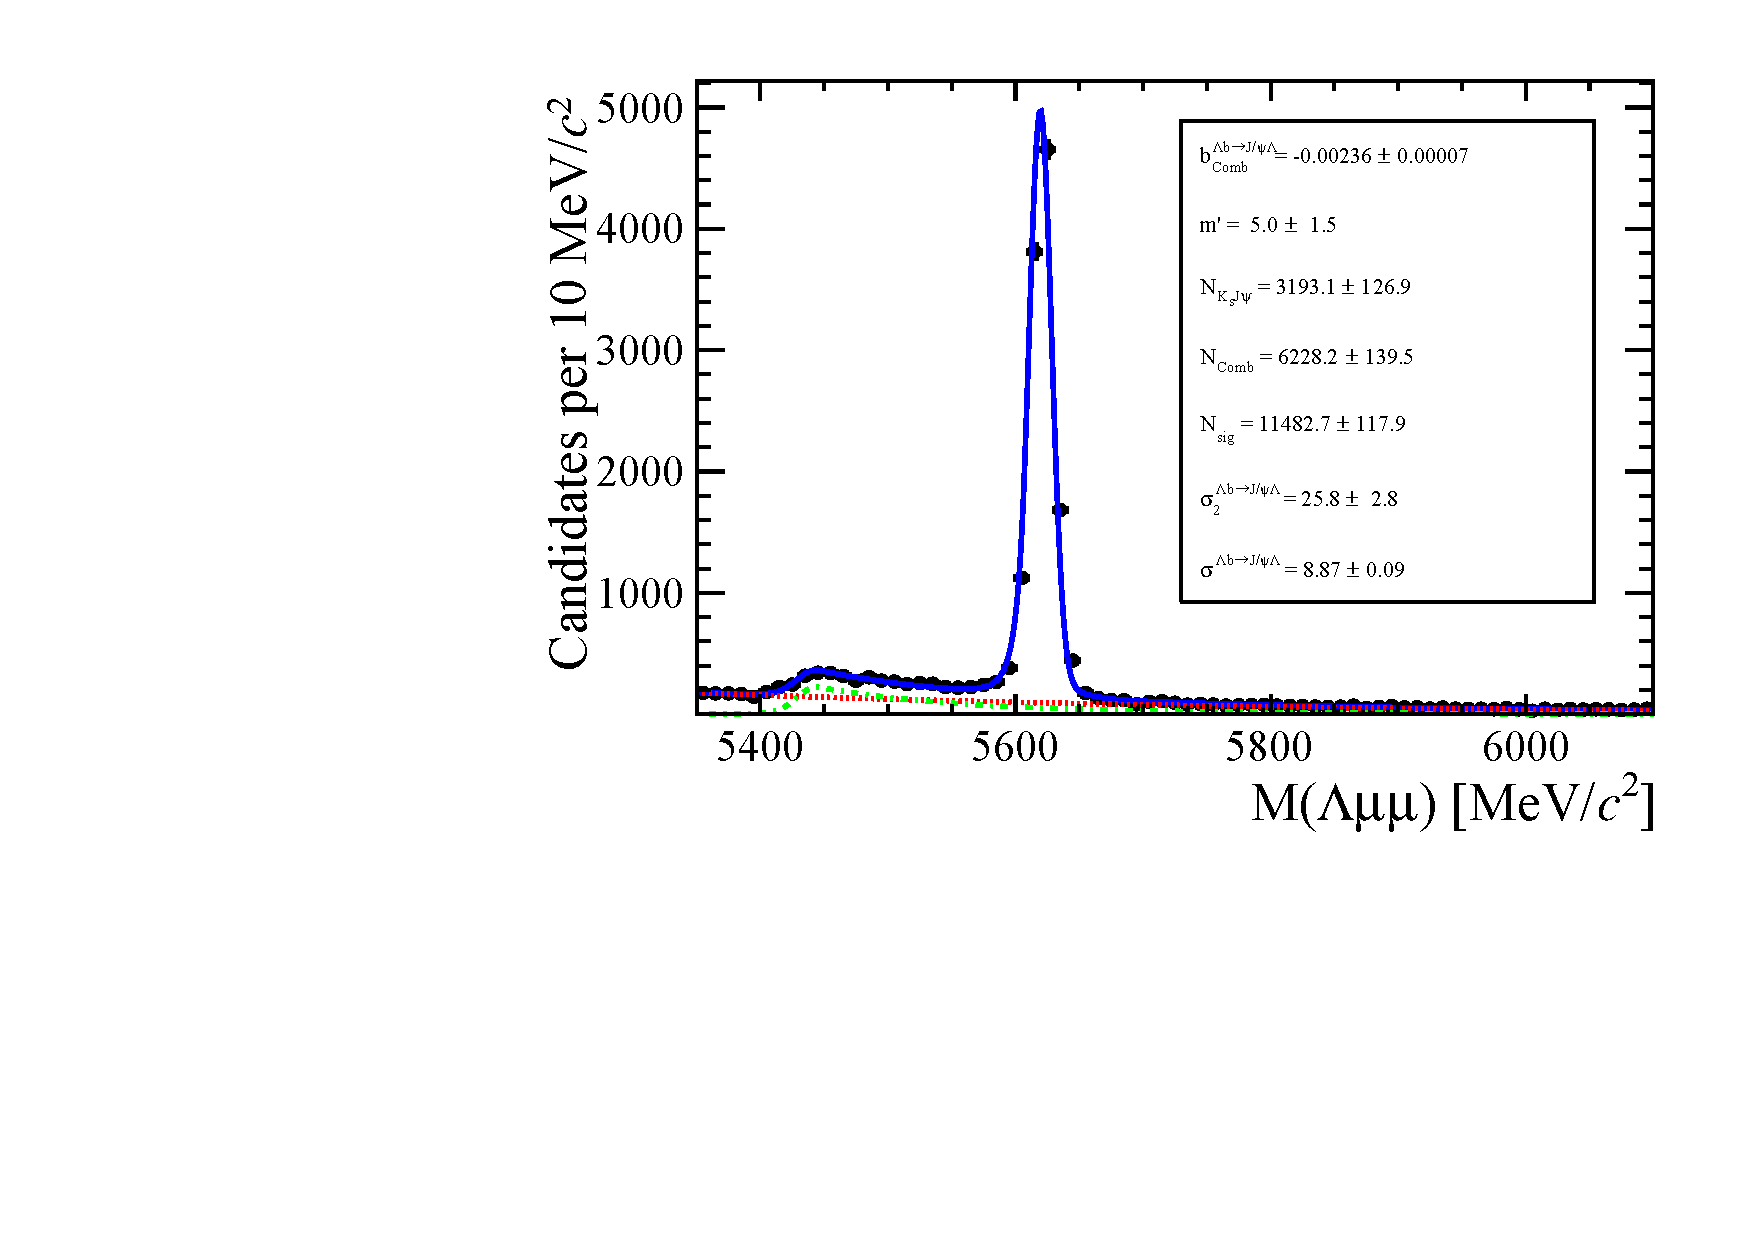
\includegraphics[width=0.75\textwidth]{Lmumu/figs/MassFits/Lb2JpsiL__DD_data.pdf}
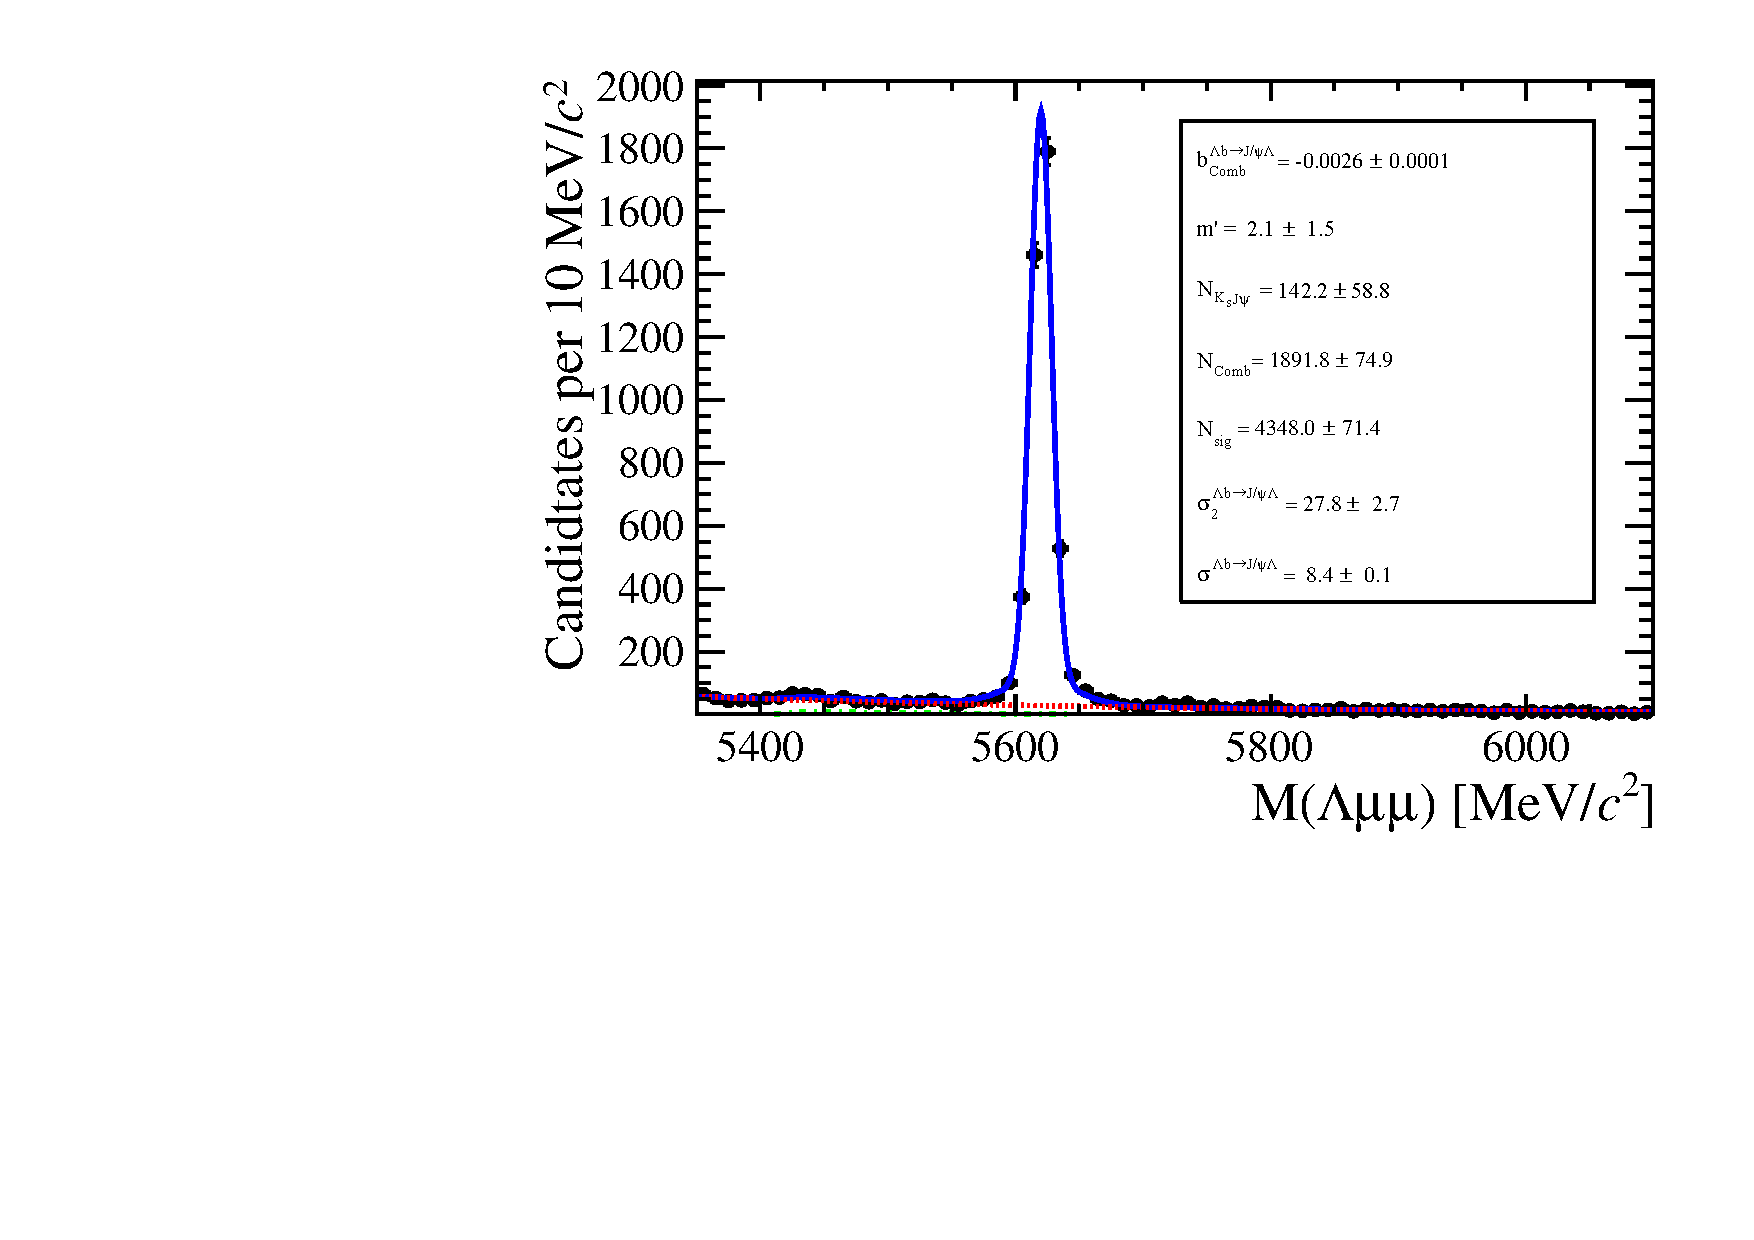
\includegraphics[width=0.75\textwidth]{Lmumu/figs/MassFits/Lb2JpsiL__LL_data.pdf}
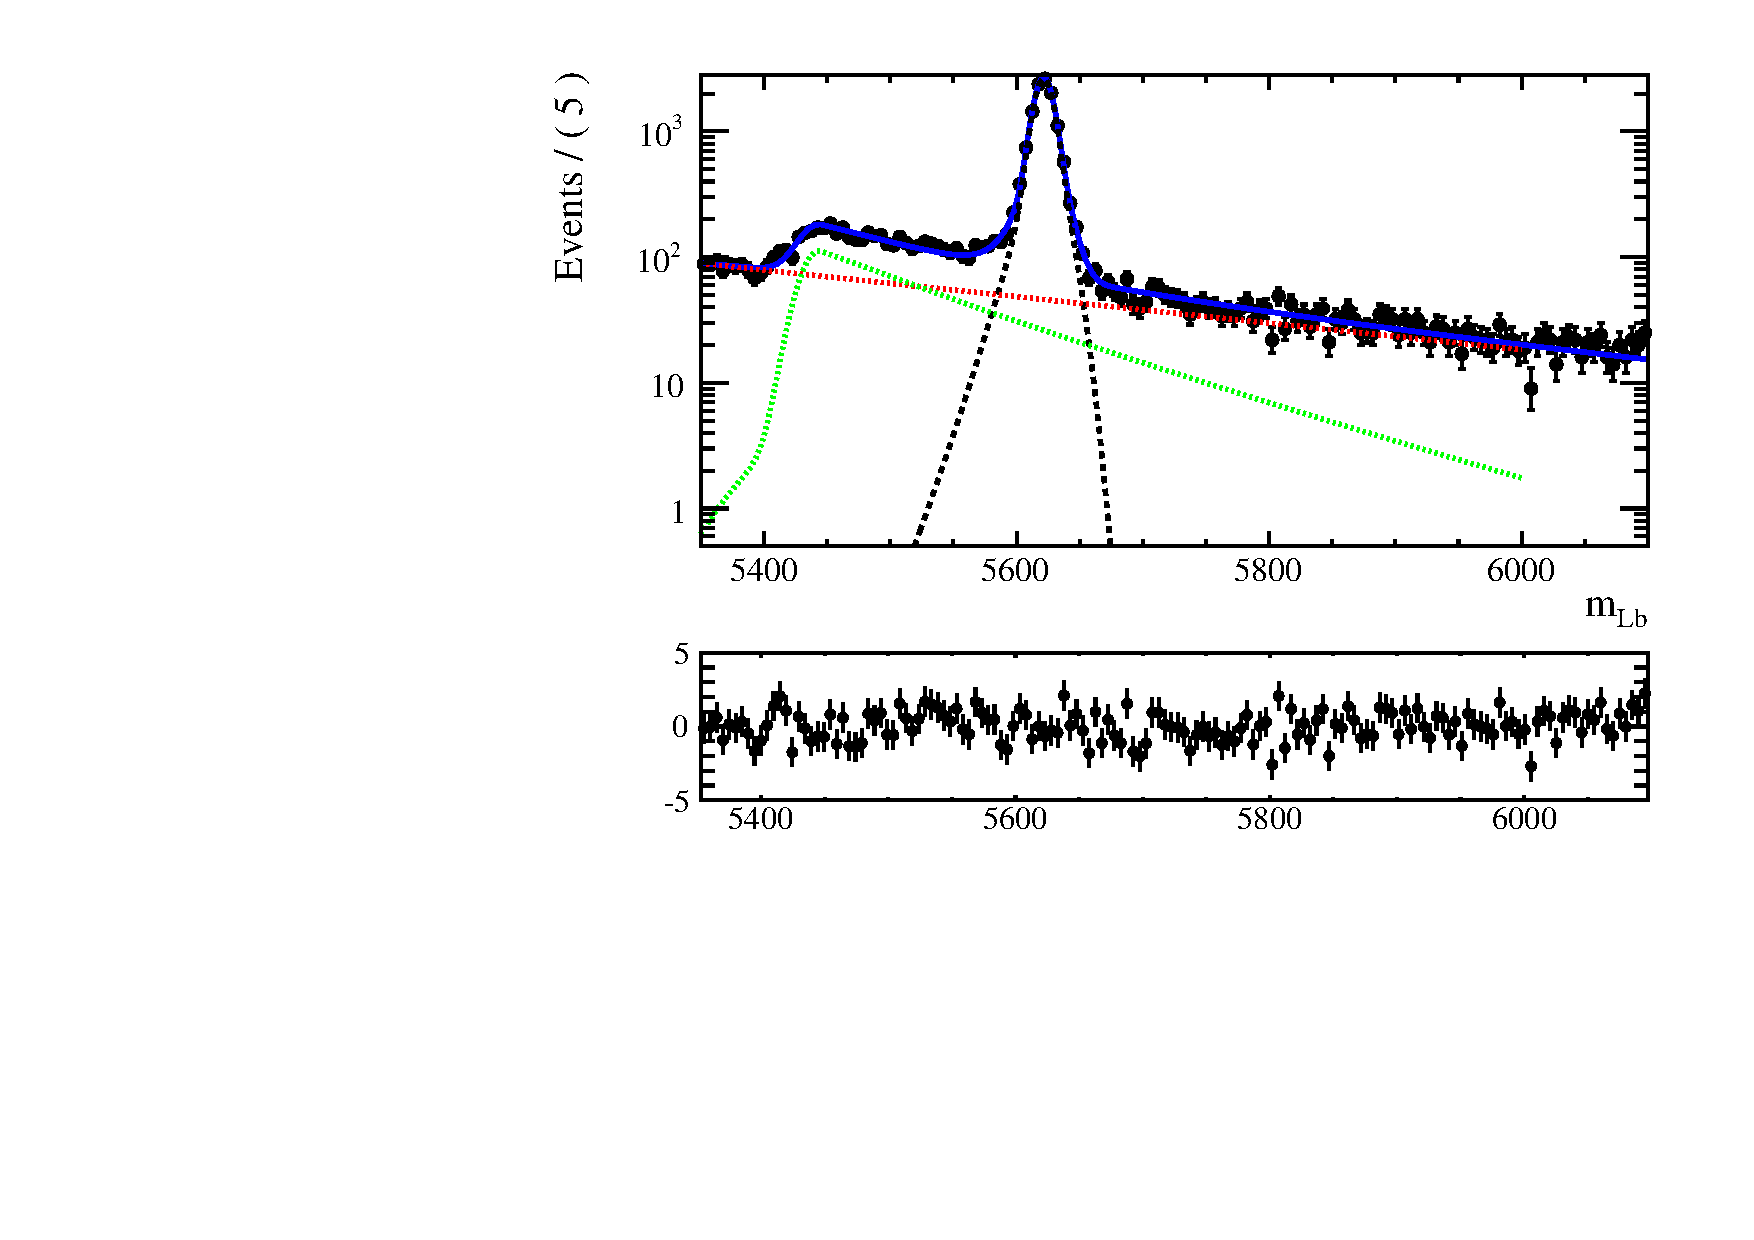
\includegraphics[width=0.49\textwidth]{Lmumu/figs/MassFits/Lb2JpsiL_DD_data_log_fitAndRes.pdf}
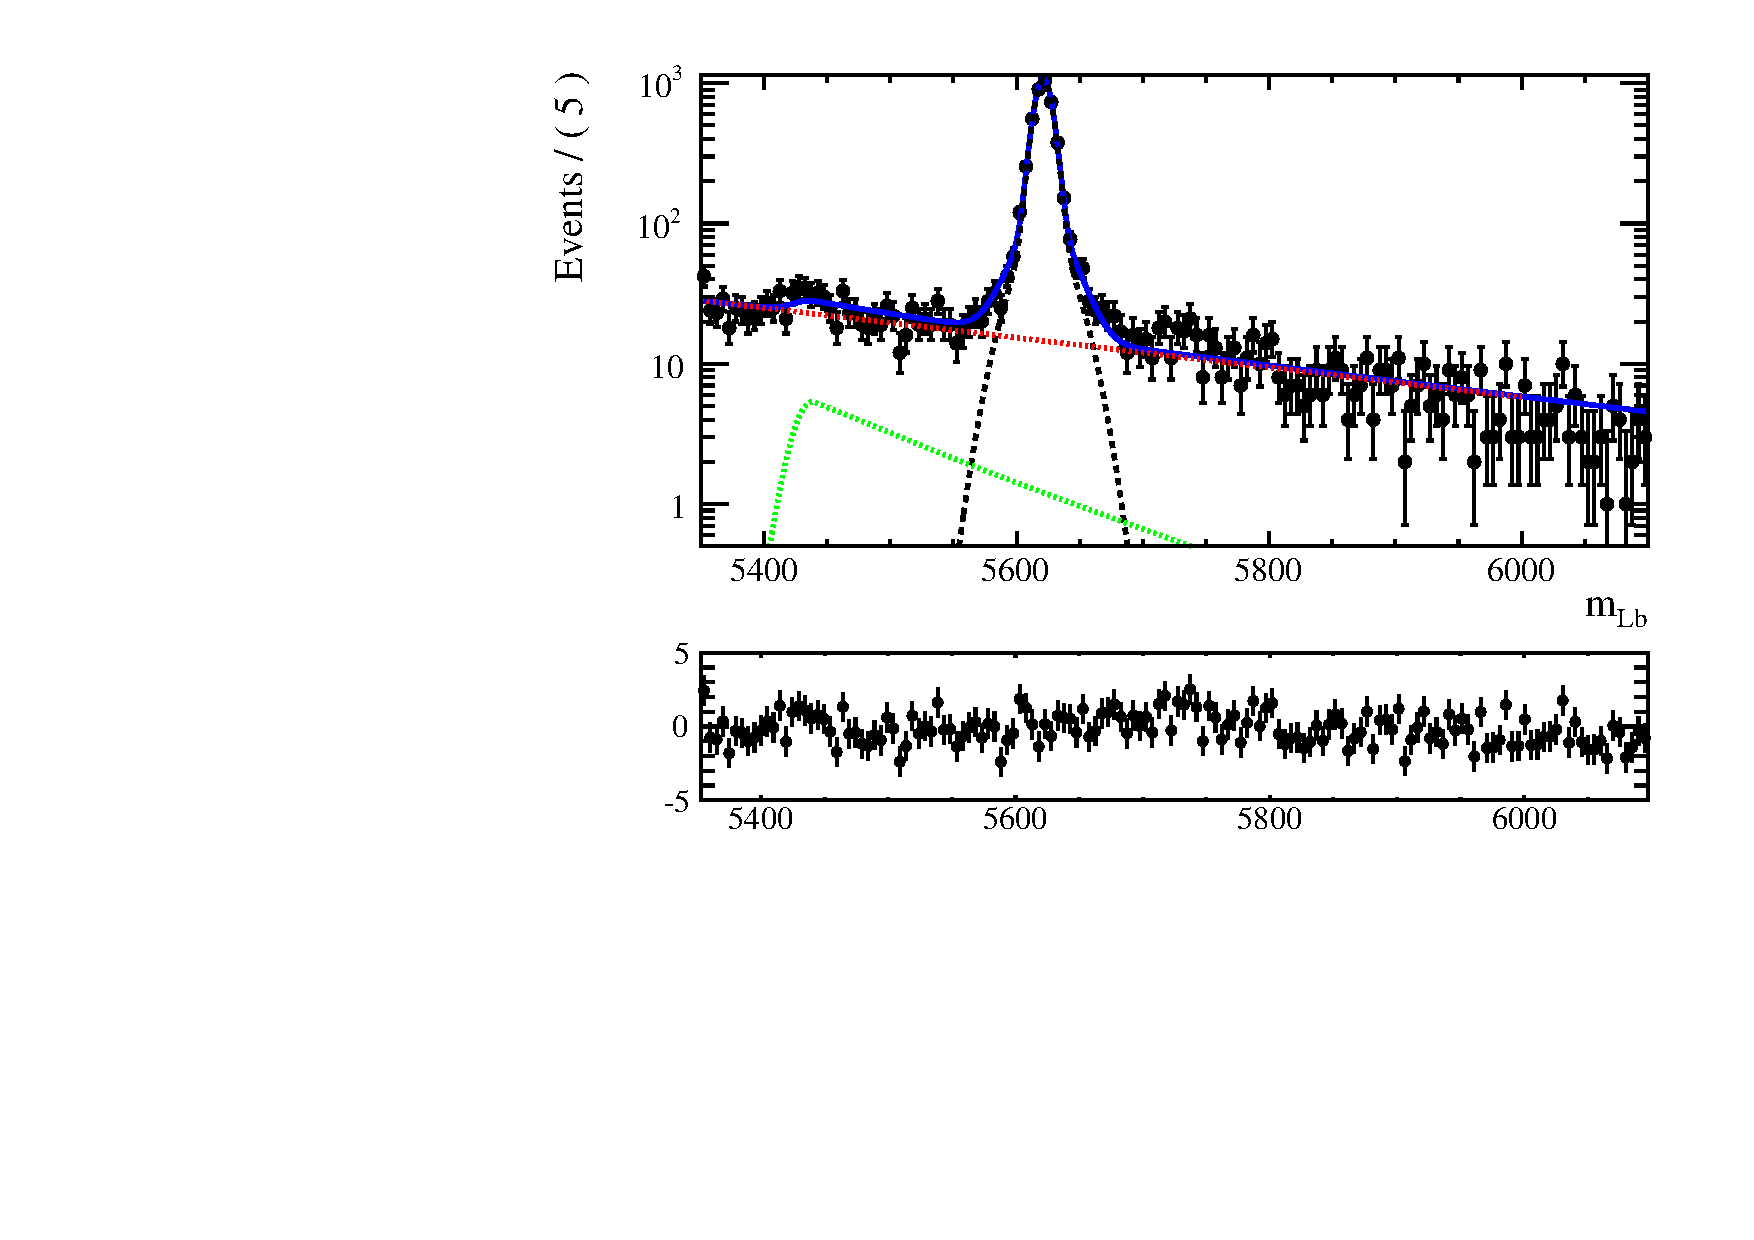
\includegraphics[width=0.49\textwidth]{Lmumu/figs/MassFits/Lb2JpsiL_LL_data_log_fitAndRes.pdf}
\caption{Invariant mass distributions of $\Lb\ra\jpsi\Lz$ downstream (top) and long (middle) candidates
selected with high \qsq requirements.
Bottom plots are the same as the upper ones but shown in logarithmic scale. Black points show data.
The blue solid line represents the total fit function, the black dashed line the signal, the red dashed line
the combinatorial background and the green dashed line the $\Bz\ra\KS\mumu$ background.}
\label{fig:Lb_totalFit}
\end{figure}
%
Figures~\ref{fig:Lb_totalFit} and~\ref{fig:Lb_totalFit_low} show fitted invariant mass distributions for
the normalisation channel, selected with the high \qsq and low \qsq requirements respectively.
%The $\chi^2$ value of the fit is $126$ for LL and $112$ for DD both with 140 degrees of freedom, which corresponds to probability of 80\% and 95\%.
Table~\ref{tab:Lb_rawYieldJpsi} reports the measured yields of $\Lb\ra\jpsi\Lz$ candidates found using the low 
and high \qsq selections. Values for the signal shape parameters are shown on Fig.~\ref{fig:Lb_totalFit}.
Fits to the rare $\Lb\ra\Lz\mumu$ samples are shown in Fig.~\ref{fig:Lb_Lmumu} for the integrated
$15 < \qsq < 20$ and $1.1 < \qsq < 6.0$~\gevgevcccc ~\qsq intervals, while
%The exponential slopes, the scale factors multiplied to the widths and the number of combinatorial events
%found from these fits are reported in Tab.~\ref{tab:Lb_rareParam}.
fitted invariant mass distribution in all other considered \qsq intervals are in Figs.~\ref{fig:Lb_differentialFitDD}
and~\ref{fig:Lb_differentialFitLL} for downstream and long candidates respectively.
The yields of rare candidates obtained from the fit are listed in Tab.~\ref{tab:Lb_rawYield} together with their significances.
Most candidates are found in the downstream sample, which comprises $\sim 80\,\%$ of the total yield.
Note that, since the fit is simultaneous to the two candidate categories, their yields
are not parameters free to float independently in the fit but are correlated via the branching ratio.
The statistical significance of the observed signal yields is evaluated as $\sqrt{2\Delta\ln{\mathcal{L}}}$, where
$\Delta\ln{\mathcal{L}}$ is the change in the logarithm of the likelihood function when the signal component
is excluded from the fit, relative to the nominal fit in which it is present.

\begin{table}
\centering
\caption{Number of \decay{\Lb}{\jpsi\Lz} candidates in the long and
  downstream categories found using the for low- and
  high-\qsq requirements. Uncertainties shown are statistical only.}
\begin{tabular}{$l^c^c}
\rowstyle{\bfseries}
Selection & Long & Downstream					\\ \hline
high-\qsq	& $4313 \pm 70$	 	&  $11\,497 \pm 123$ \\
low-\qsq	& $3363 \pm 59$ 	&  $\phantom{0}\,7225 \pm 89\phantom{0}$  \\
 \hline
\end{tabular}
\label{tab:Lb_rawYieldJpsi}
\end{table}

\begin{table}
\centering
\caption{Signal yields ($N_\mathrm{S}$) obtained from the
  mass fit to \decay{\Lb}{\Lz\mumu} candidates in each \qsq interval
  together with their statistical significances. 
  The $8-11$ and $12.5-15$ \gevgevcccc ~\qsq intervals are excluded
  from the study as they are dominated by decays via charmonium resonances.}
\begin{tabular}{$l^c^c^c^c}
\rowstyle{\bfseries} 
 \qsq interval [\gevgevcccc] & DD & LL & Tot. yield & Significance \\ \hline
\phantom{x}0.1 -- 2.0\phantom{x}   &  $\phantom{x}6.9 \pm 2.2$  &  $\phantom{xx}9.1 \pm 3.0\phantom{x}$	 &  $16.0\pm5.3$            		&  4.4 \\
\phantom{x}2.0 -- 4.0\phantom{x}   &  $\phantom{x}1.8 \pm 1.7$  &  $\phantom{xx}3.0 \pm 2.8\phantom{x}$ 	 &  $\phantom{x}4.8\pm4.7$  	 &  1.2 \\
\phantom{x}4.0 -- 6.0\phantom{x}   &  $\phantom{x}0.4 \pm 0.9$  &  $\phantom{xx}0.6 \pm 1.4\phantom{x}$	 &  $\phantom{x}0.9\pm2.3$  	 &  0.5 \\
\phantom{x}6.0 -- 8.0\phantom{x}   &  $\phantom{x}4.3 \pm 2.0$   &  $\phantom{xx}7.2 \pm 3.3\phantom{x}$	 &  $11.4\pm5.3$            		&  2.7 \\
11.0 -- 12.5  				     &  $14.6 \pm 2.9$  		    &  $\phantom{x}42.8 \pm 8.5\phantom{x}$  &  $\phantom{x.}60\pm12\phantom{.}$ &  6.5 \\
15.0 -- 16.0  			             &  $13.5 \pm 2.2$  		    &  $\phantom{x}43.5 \pm 7.2\phantom{x}$   &  $\phantom{x.}57\pm9\phantom{x.}$             			 &  8.7 \\
16.0 -- 18.0  				    &  $28.6 \pm 3.3$  		    &  $\phantom{x}88.8 \pm 10.1$	 	       &  $\phantom{.}118\pm13\phantom{.}$              			 &  13  \\
18.0 -- 20.0  				    &  $22.4 \pm 2.6$  		    &  $\phantom{x}78.0 \pm 8.9\phantom{x}$ &  $\phantom{.}100\pm11\phantom{.}$    &  14  \\
\hline
\phantom{x}1.1 -- 6.0\phantom{x}    	&  $\phantom{x}3.6 \pm 2.4$  &  $\phantom{xx}5.7 \pm 3.8\phantom{x}$	 &  $\phantom{x}9.4\pm6.3$  			&  1.7 \\
15.0 -- 20.0  					&  $64.6 \pm 4.7$  			&  $209.6 \pm 15.3$ 					&  $\phantom{.}276\pm20\phantom{.}$              		&  21  \\
\end{tabular}
\label{tab:Lb_rawYield}
\end{table}

\begin{figure}
\centering
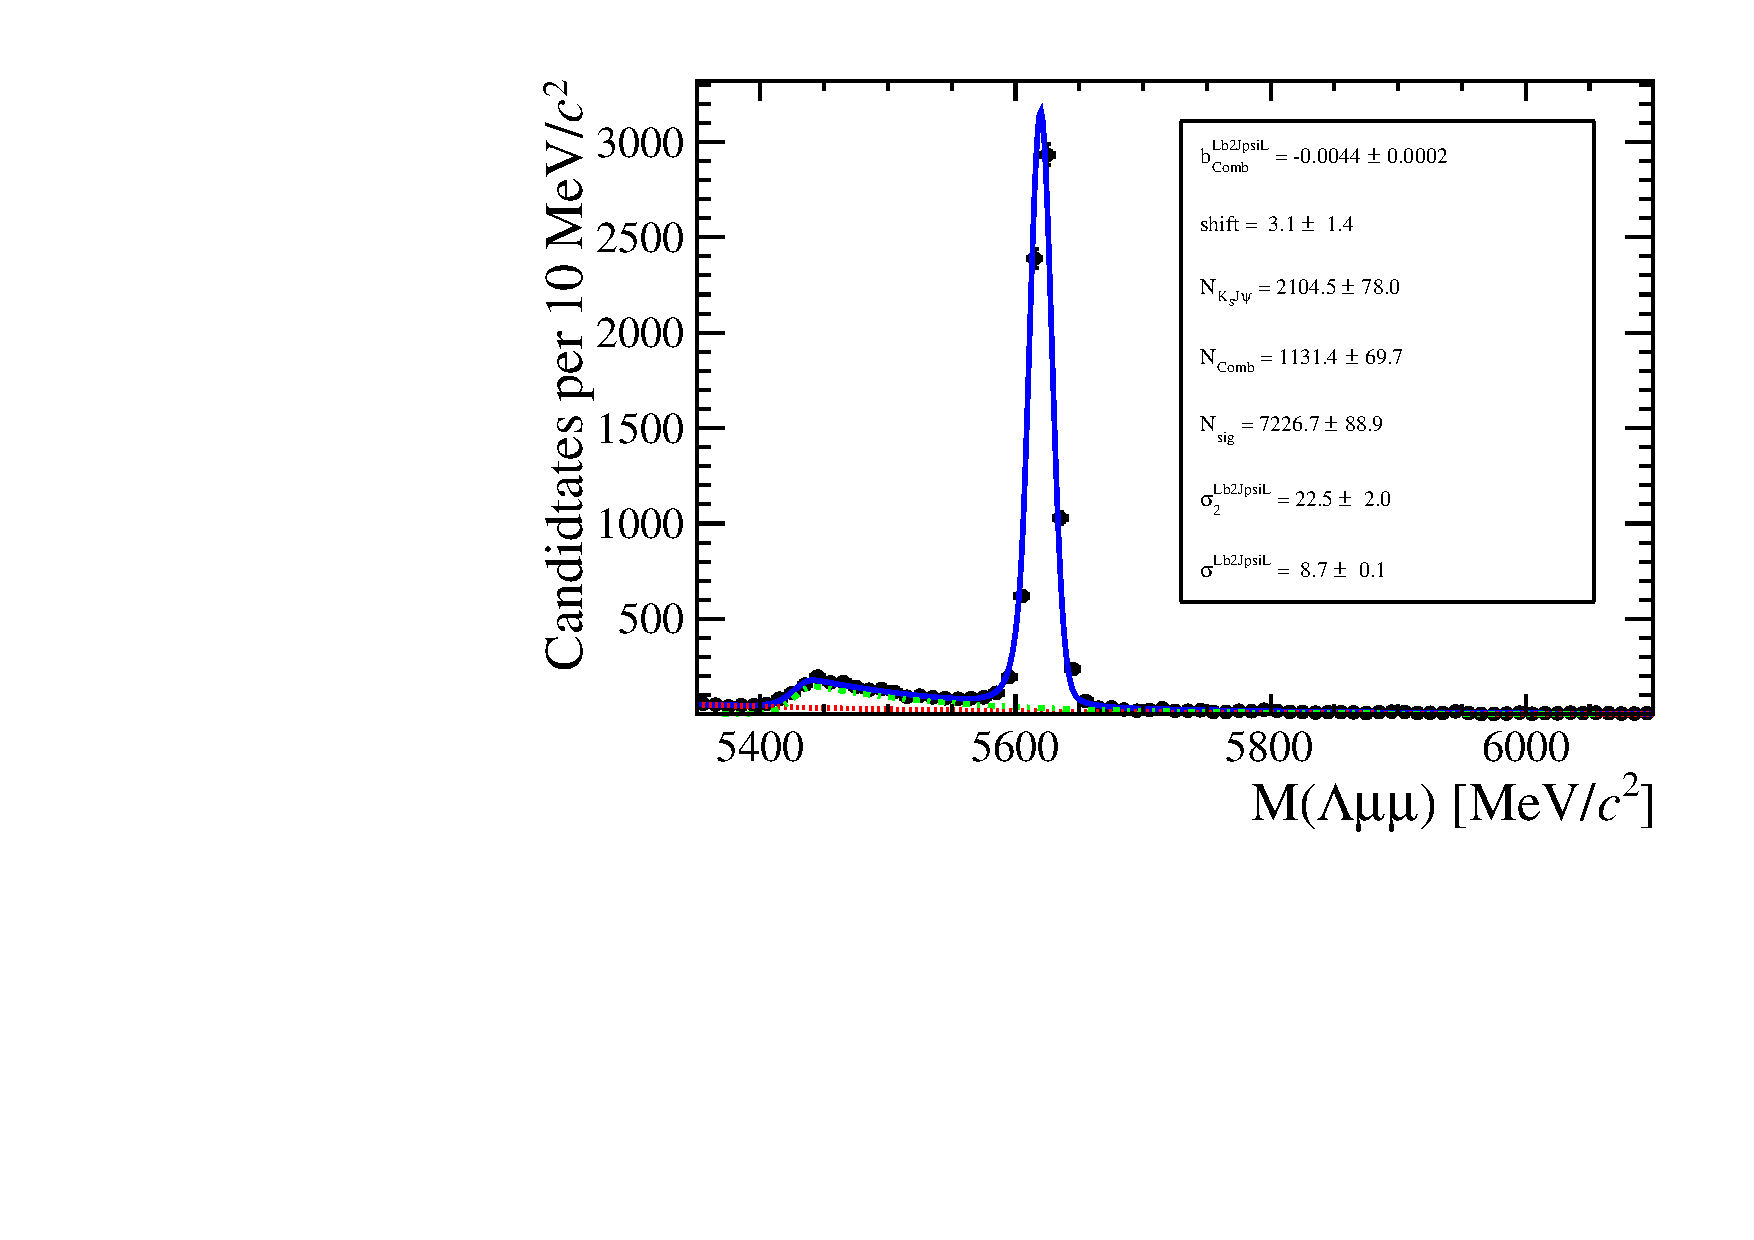
\includegraphics[width=0.49\textwidth]{Lmumu/figs/MassFits/Lb2JpsiL__lowSel_DD_data.pdf}
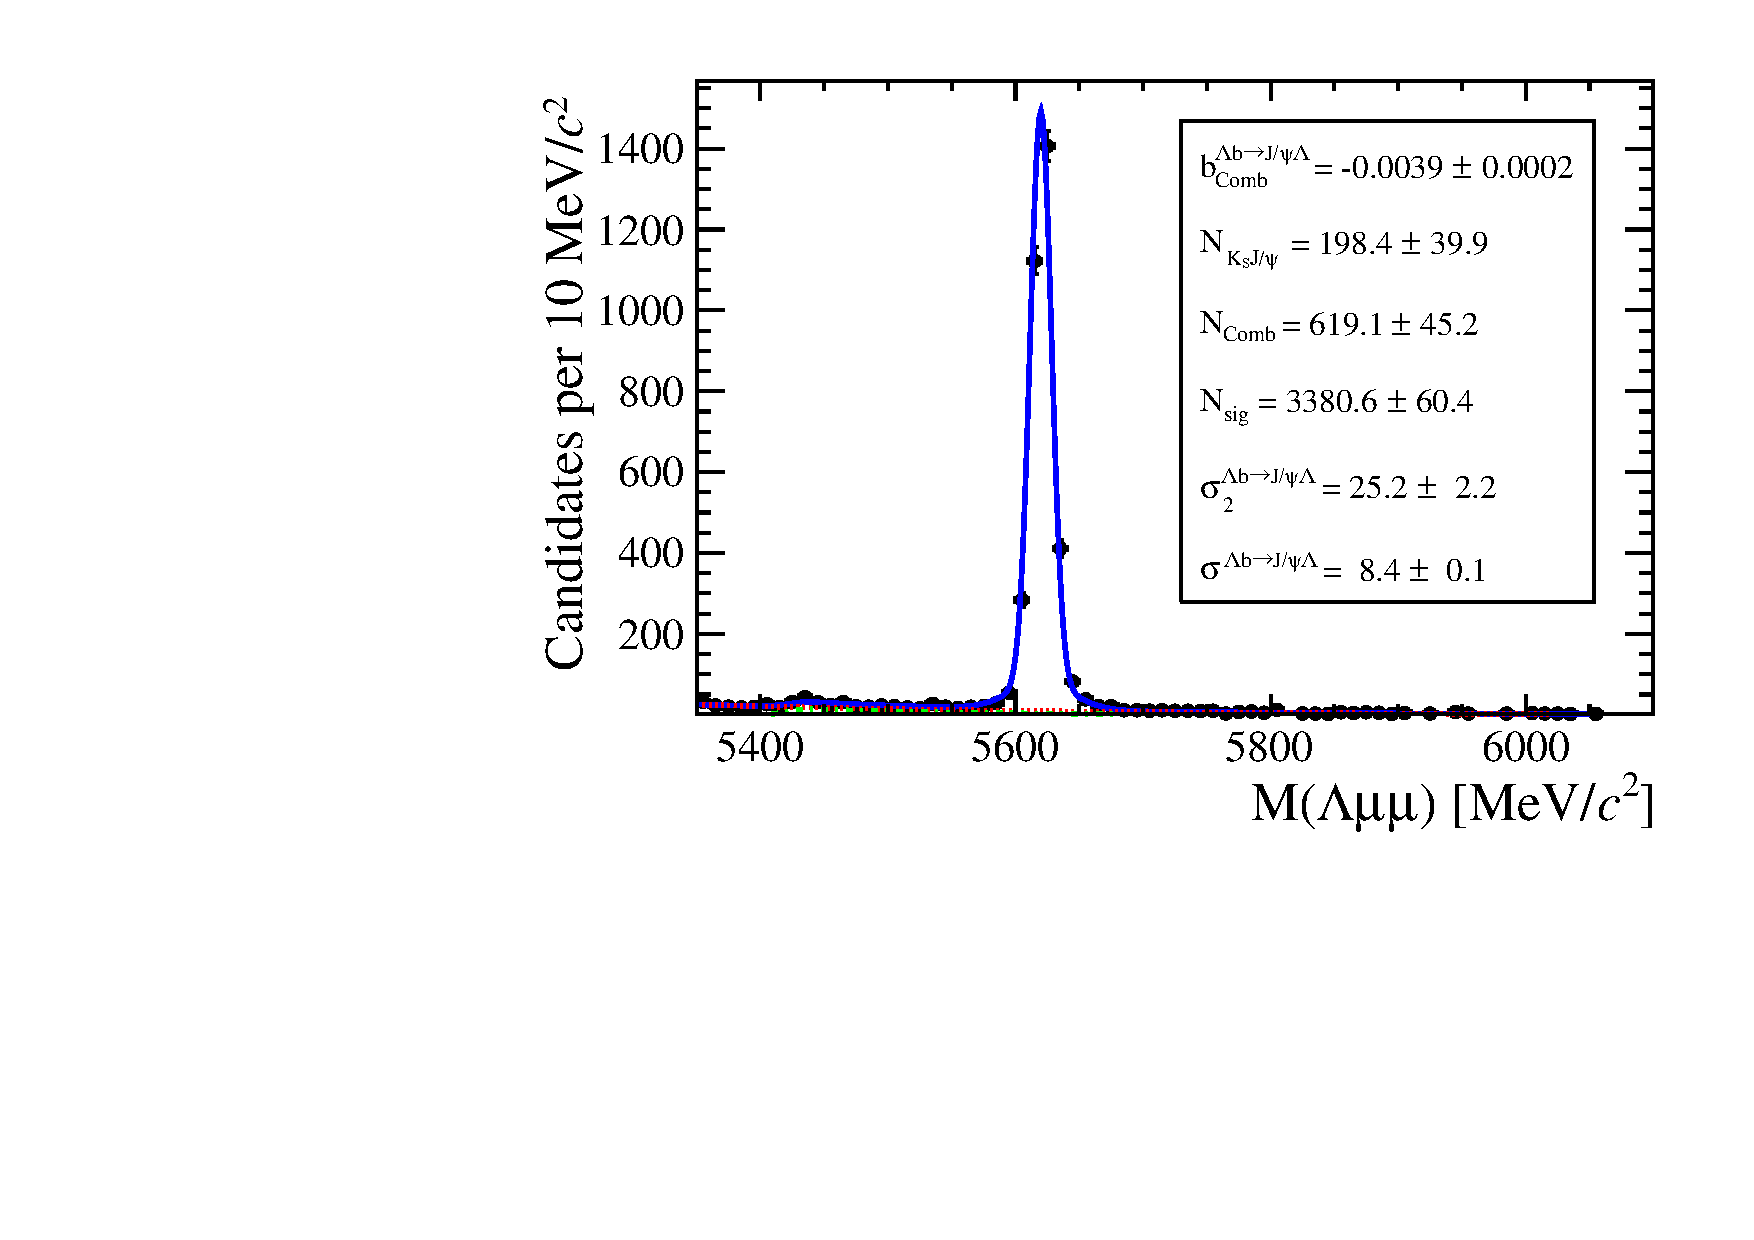
\includegraphics[width=0.49\textwidth]{Lmumu/figs/MassFits/Lb2JpsiL__lowSel_LL_data.pdf}
\caption{Invariant mass distribution of $\Lb\ra\jpsi\Lz$ for downstream (left) and long (right) candidates
 selected with low \qsq requirements.}
\label{fig:Lb_totalFit_low}
\end{figure}
%
%
\begin{figure}
\centering
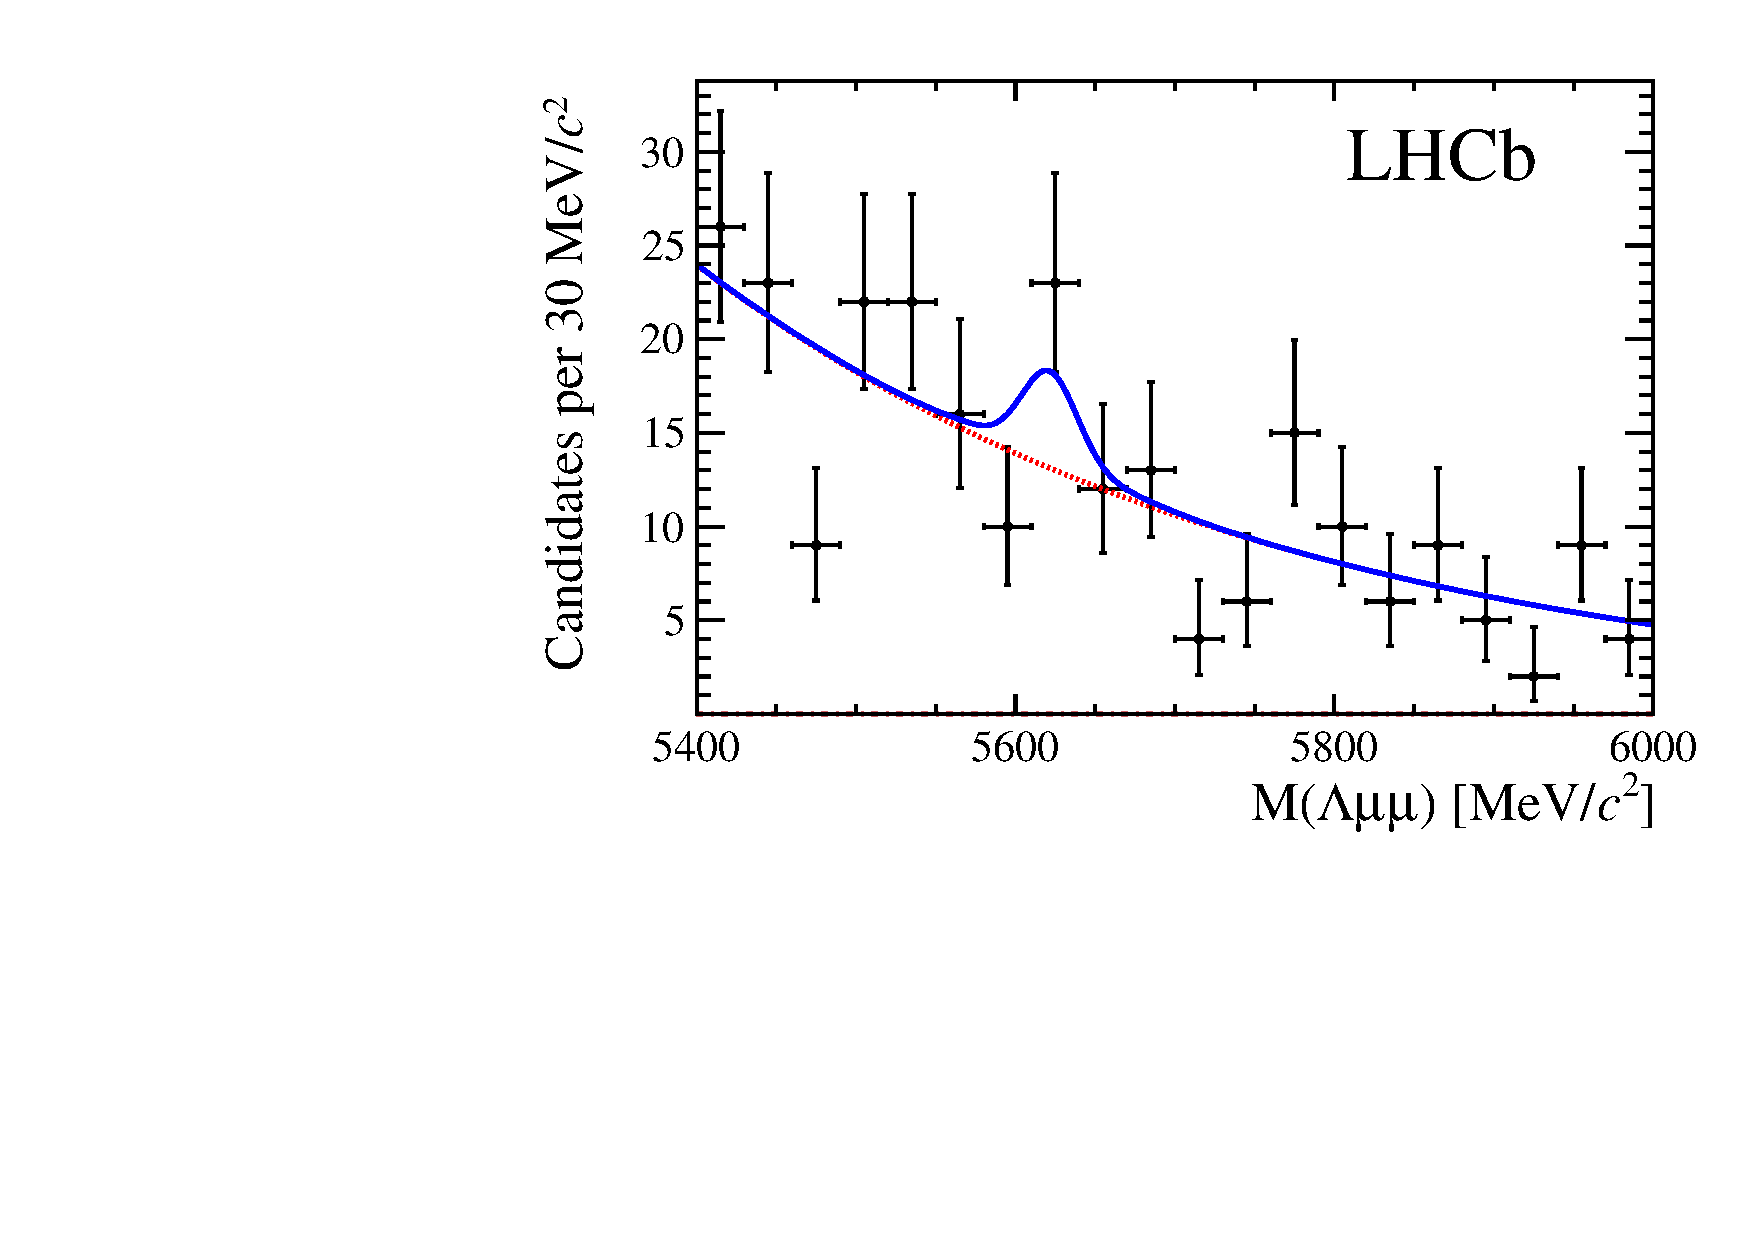
\includegraphics[width=0.7\textwidth]{Lmumu/figs/paper/figure13.pdf}
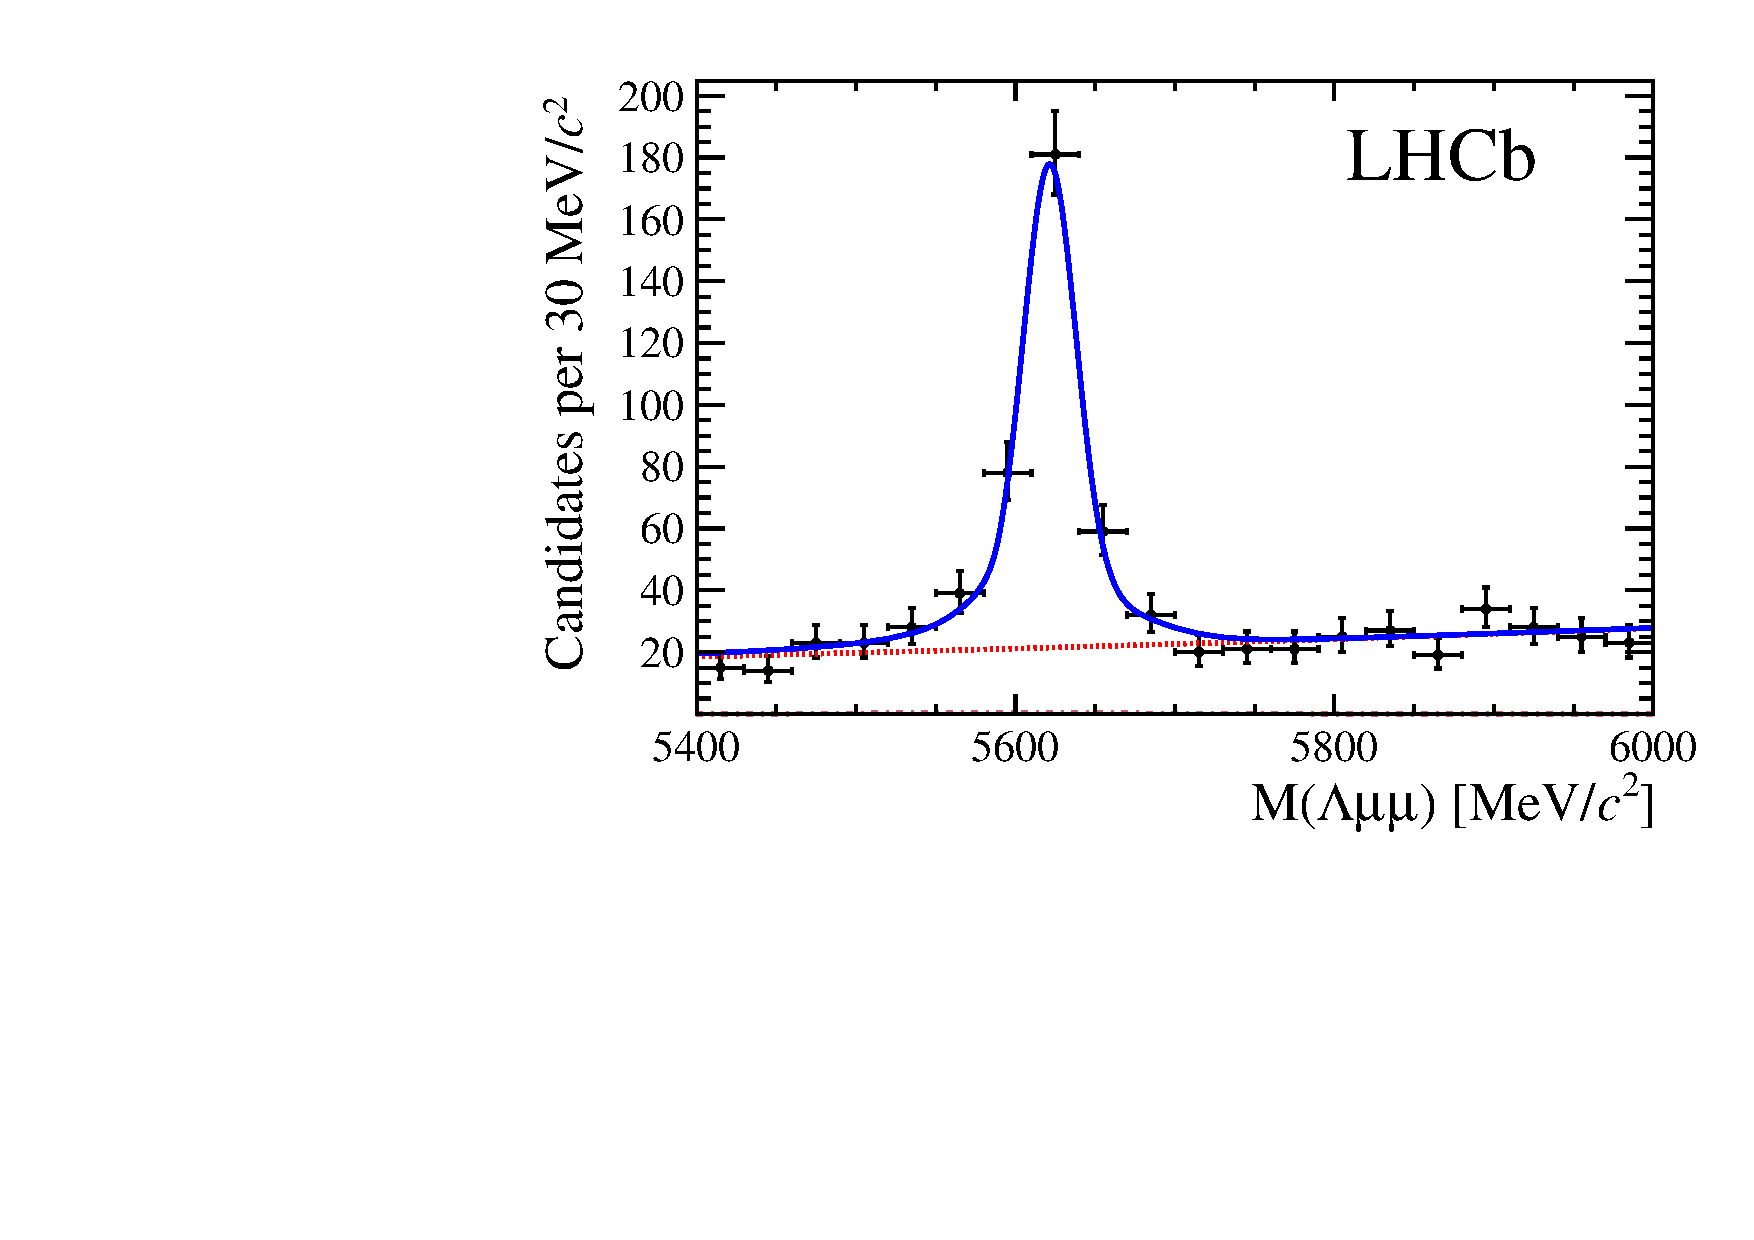
\includegraphics[width=0.7\textwidth]{Lmumu/figs/paper/figure2.pdf}
\caption{Invariant mass distributions of $\Lb\ra\Lz\mumu$ candidates in the integrated 0.1--6.0 \gevgevcccc(top)
and 15--20 \gevgevcccc (bottom) ~\qsq intervals. Points show data combining downstream and long candidates together.
The blue solid line represents the total fit function and the dashed red line the combinatorial background.}
%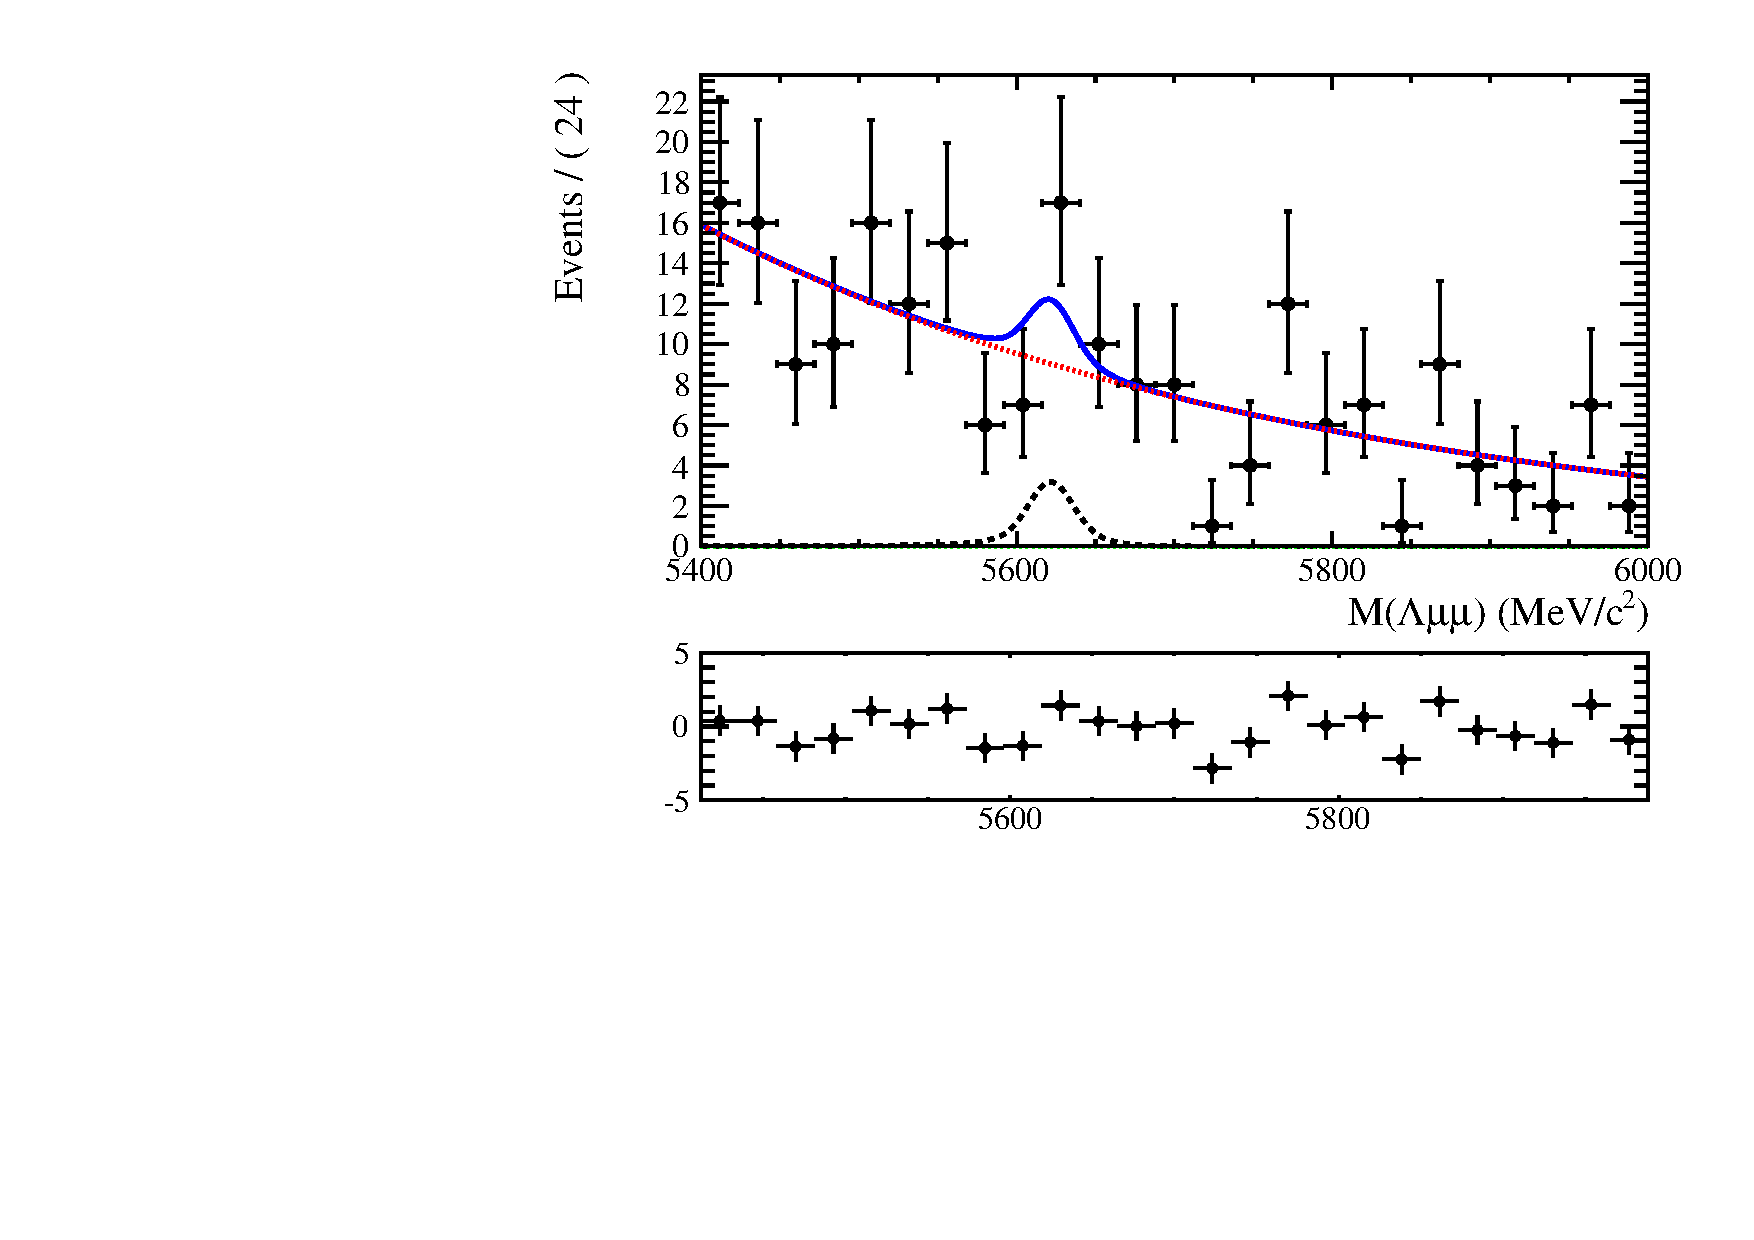
\includegraphics[width=0.54\textwidth]{Lmumu/figs/MassFits/Lb2Lmumu_DD_lowQ2_fitAndRes.pdf}
%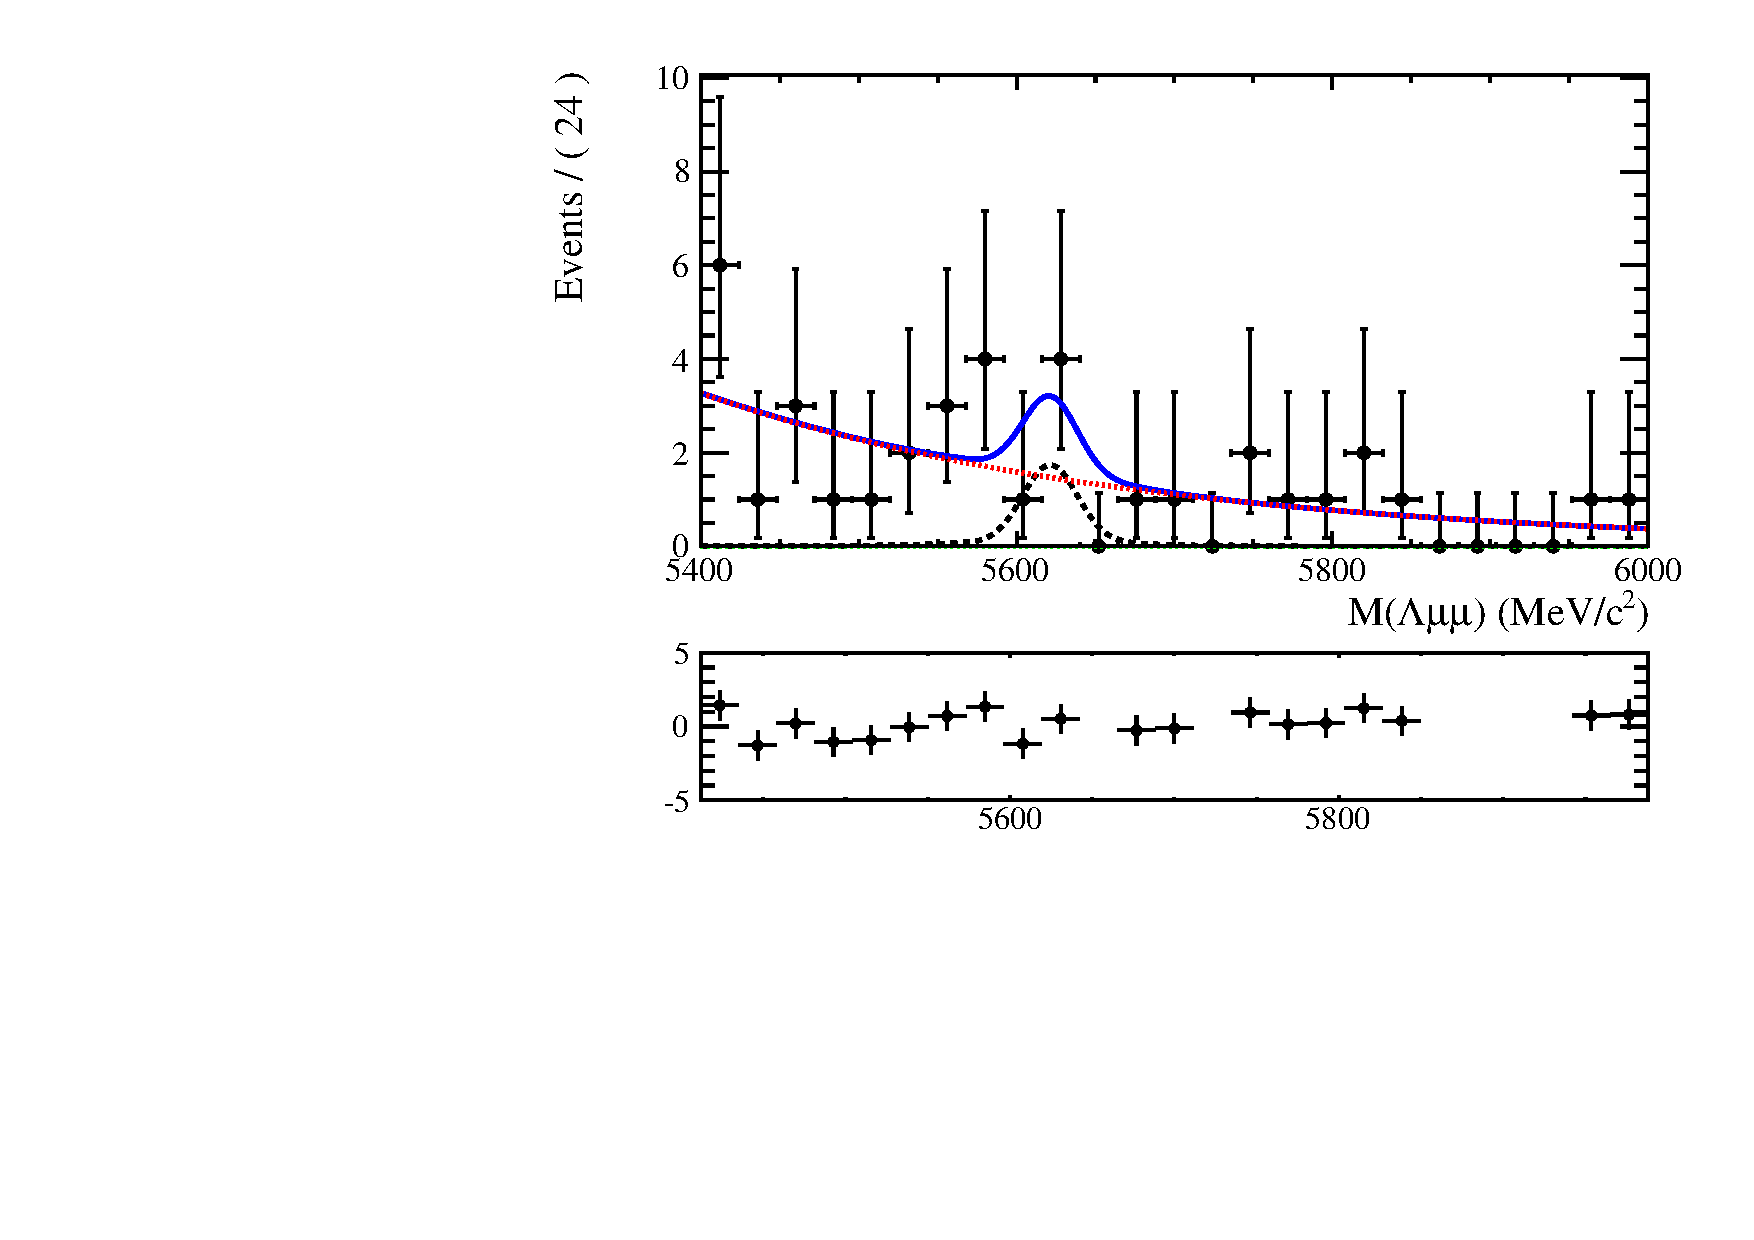
\includegraphics[width=0.54\textwidth]{Lmumu/figs/MassFits/Lb2Lmumu_LL_lowQ2_fitAndRes.pdf}
%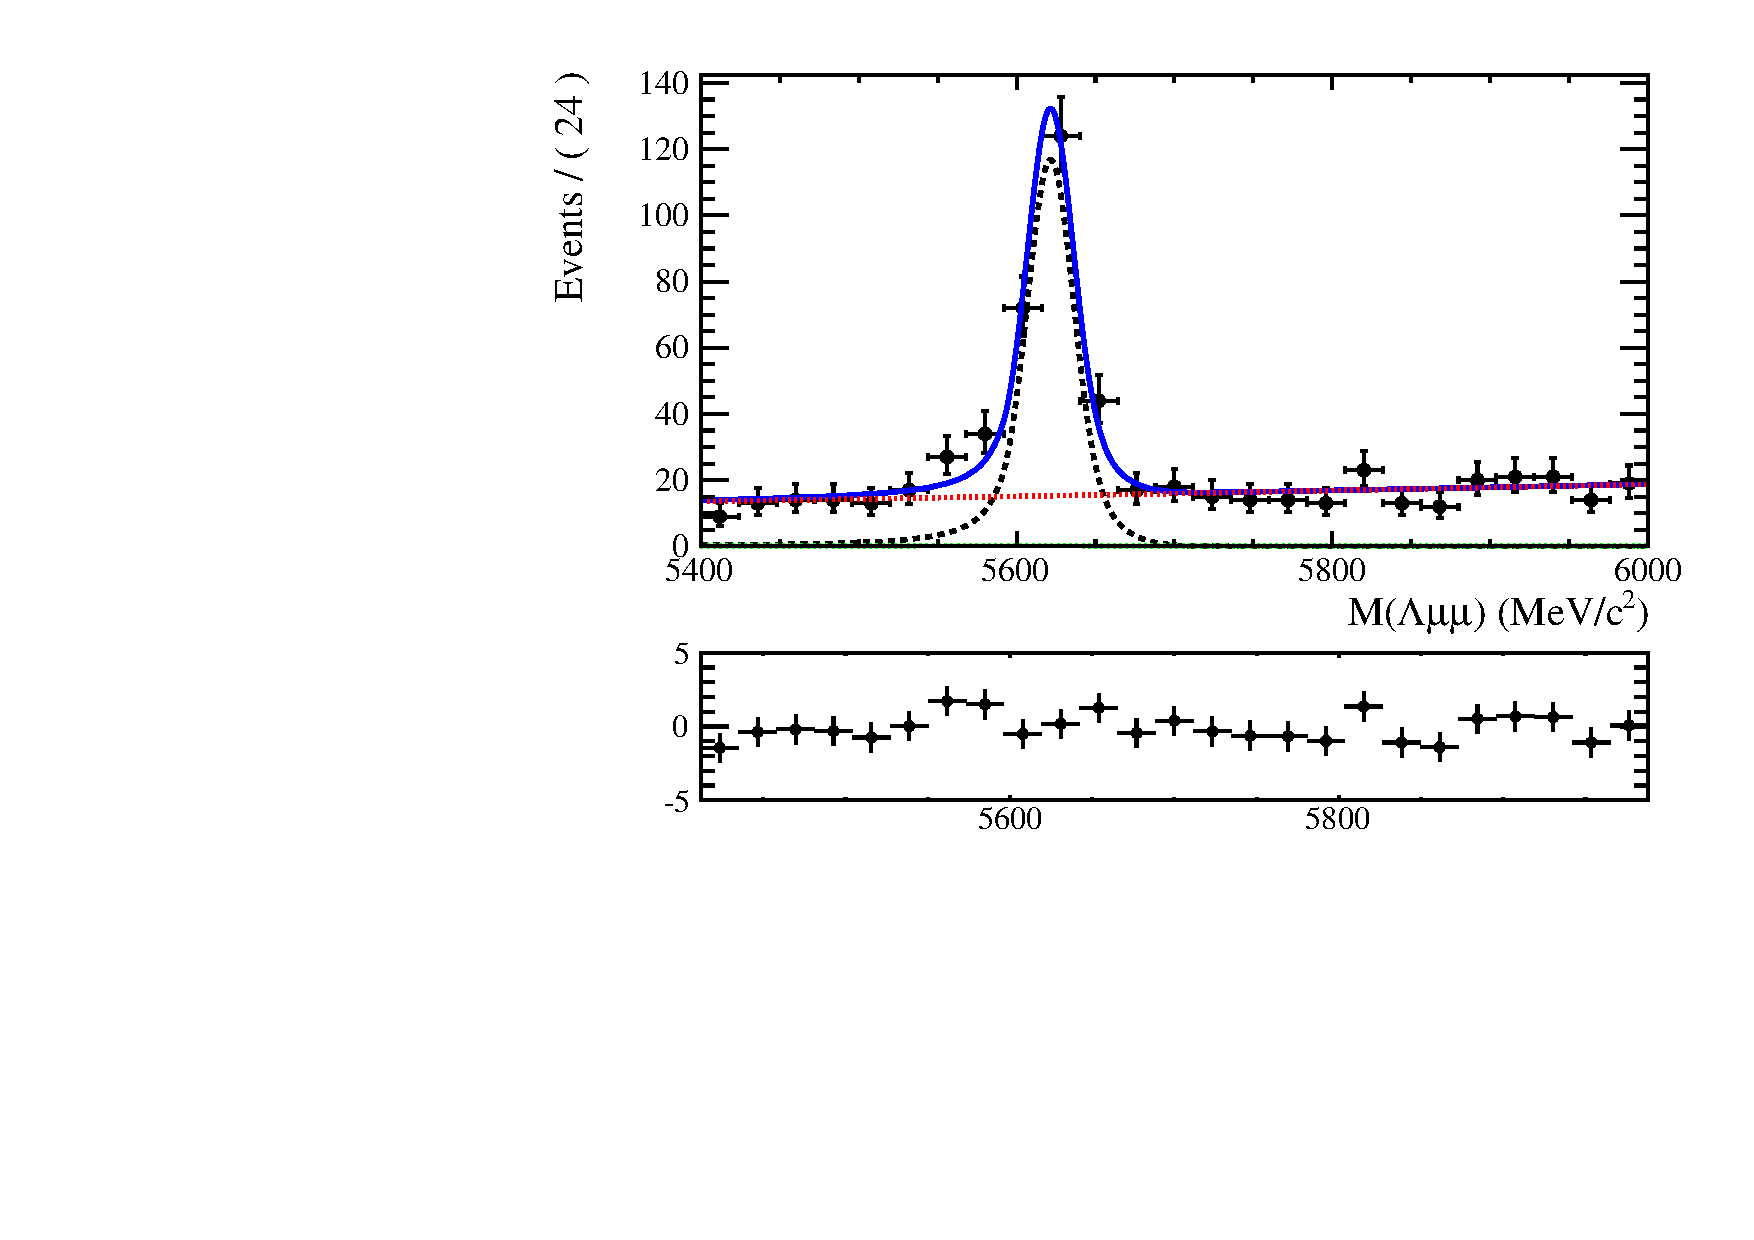
\includegraphics[width=0.54\textwidth]{Lmumu/figs/MassFits/Lb2Lmumu_DD_highQ2_fitAndRes.pdf}
%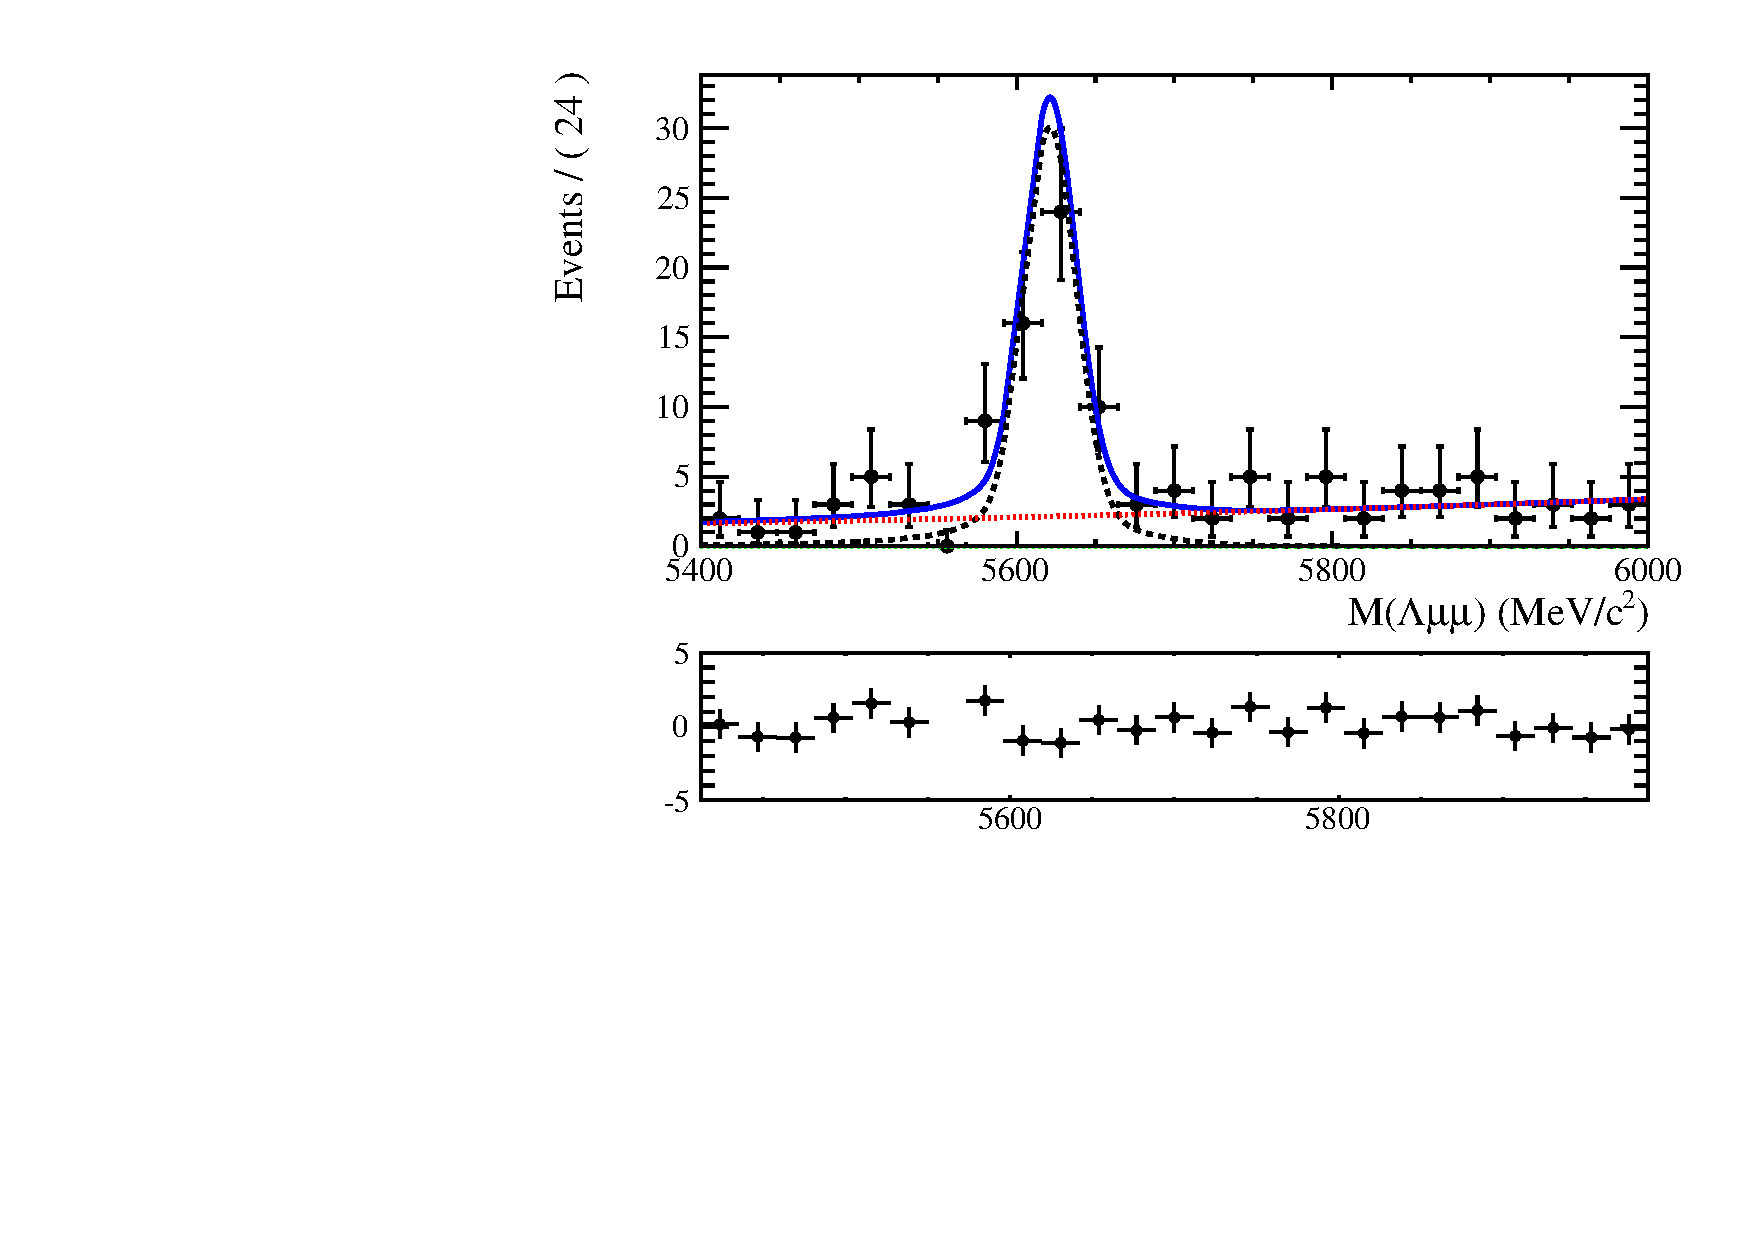
\includegraphics[width=0.54\textwidth]{Lmumu/figs/MassFits/Lb2Lmumu_LL_highQ2_fitAndRes.pdf}
%\caption{Invariant mass distribution of $\Lb\ra\Lz\mumu$ candidates in the integrated 0.1--6.0 (top)
%\gevgevcccc ~\qsq interval for downstream (left) and long (right) candidates. The points show data, the blue line
%and 15.0--20.0 (bottom) \gevgevcccc \qsq intervals.
%The blue solid line represents the total fit function and the dashed red line the combinatorial background.}
\label{fig:Lb_Lmumu}
\end{figure}
%
\begin{figure}
\centering
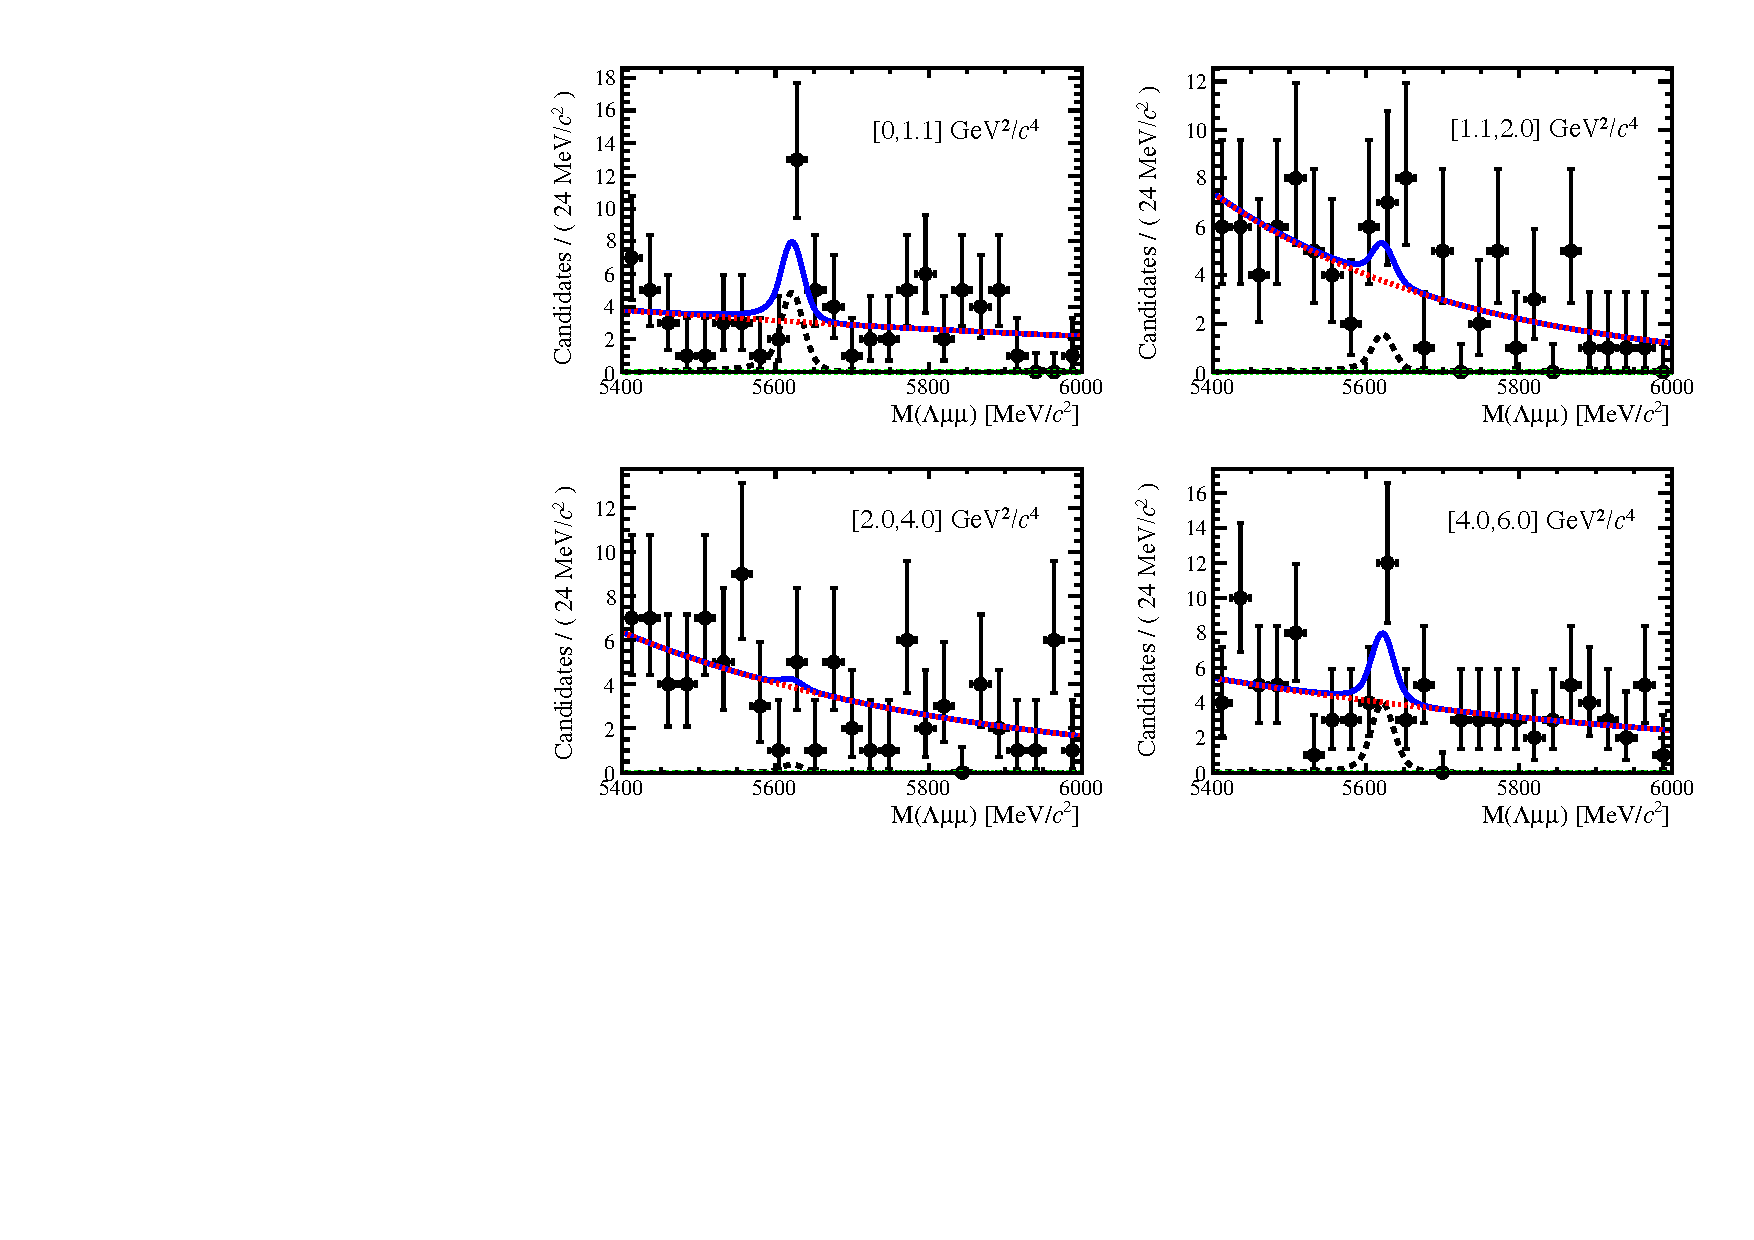
\includegraphics[width=1.\textwidth]{Lmumu/figs/MassFits/q2_fits_DD_plot2.pdf}
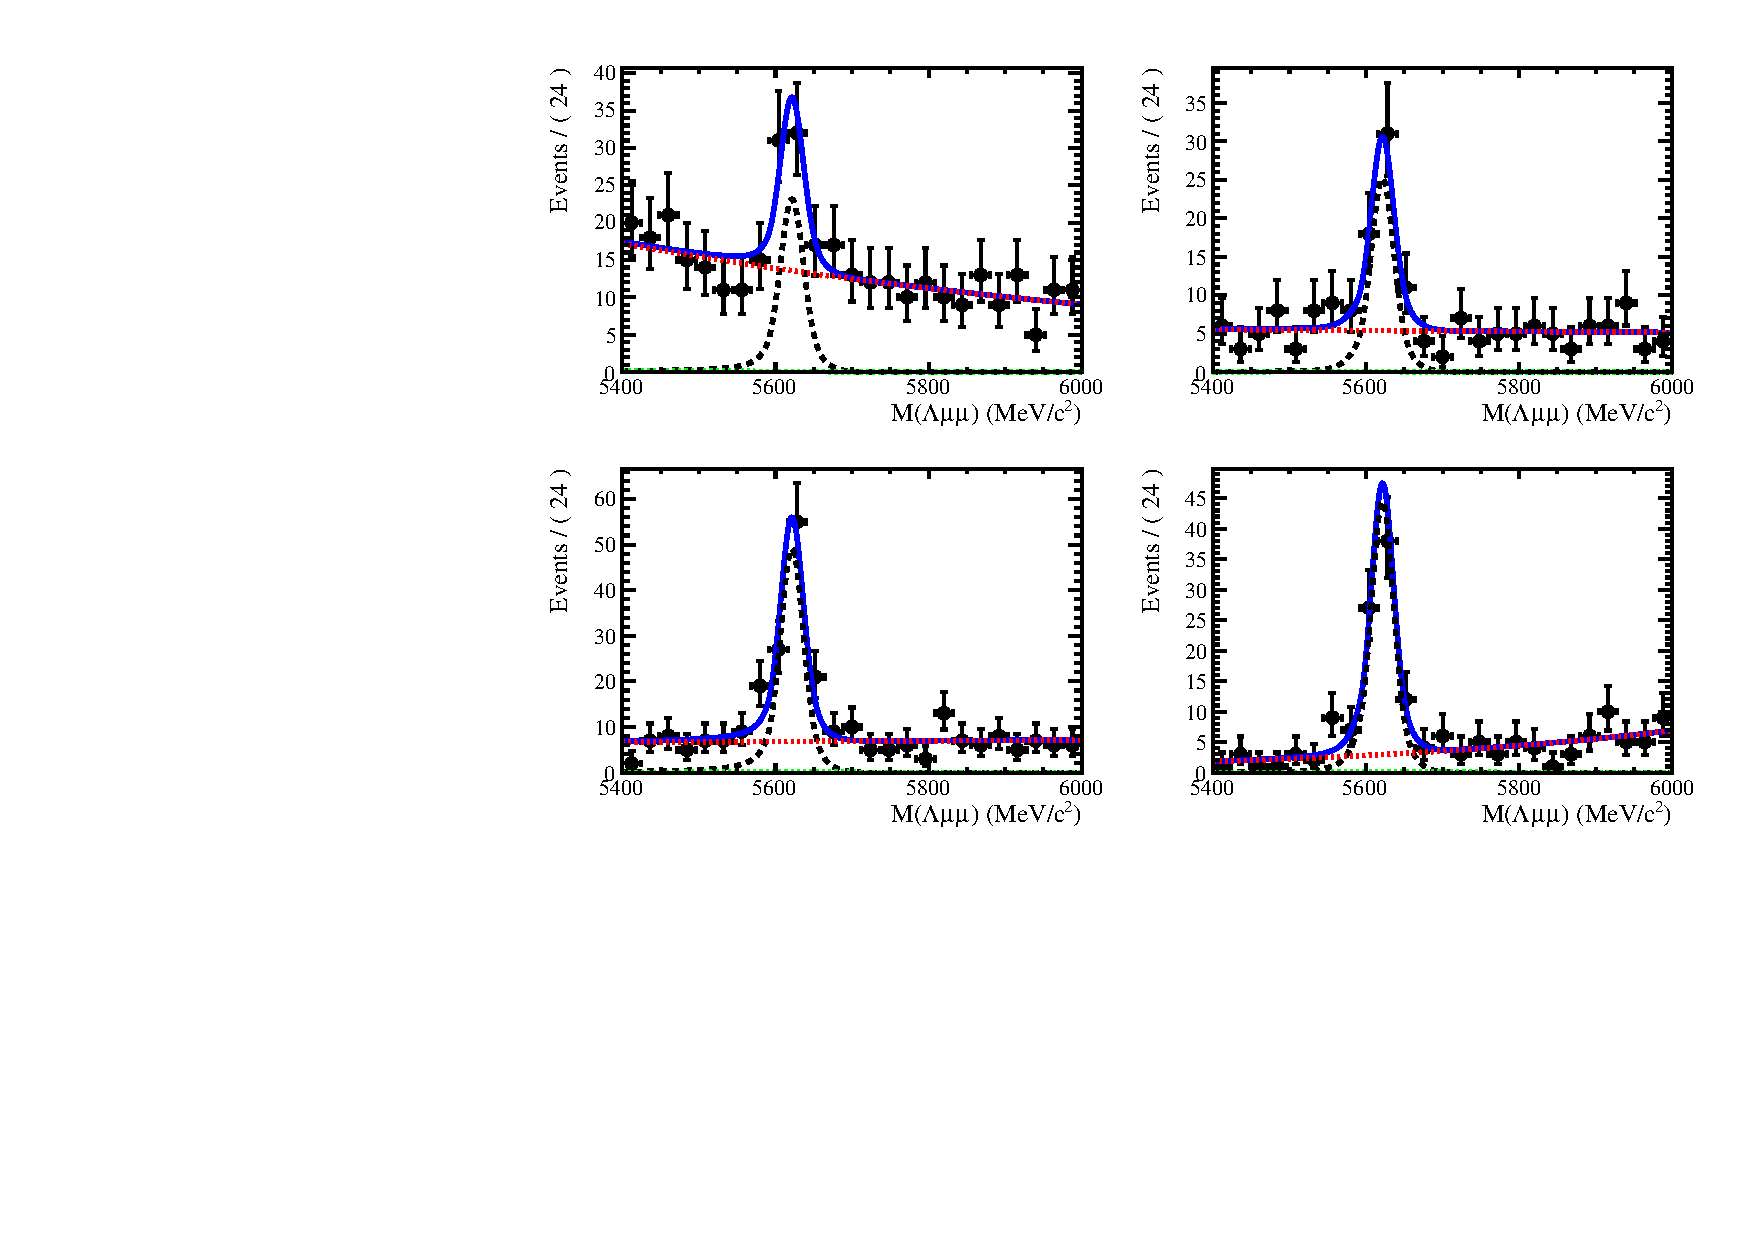
\includegraphics[width=1.\textwidth]{Lmumu/figs/MassFits/q2_fits_DD_plot1.pdf}
\caption{Invariant mass distributions of rare $\Lb\ra\Lz\mumu$ candidates in the considered \qsq bins
 %[0.1,2], [2,4], [4,6], [6,8], [11,12.5], [15,16], [16,18], [18,20]
 for downstream candidates. }
\label{fig:Lb_differentialFitDD}
\end{figure}

\begin{figure}
\centering
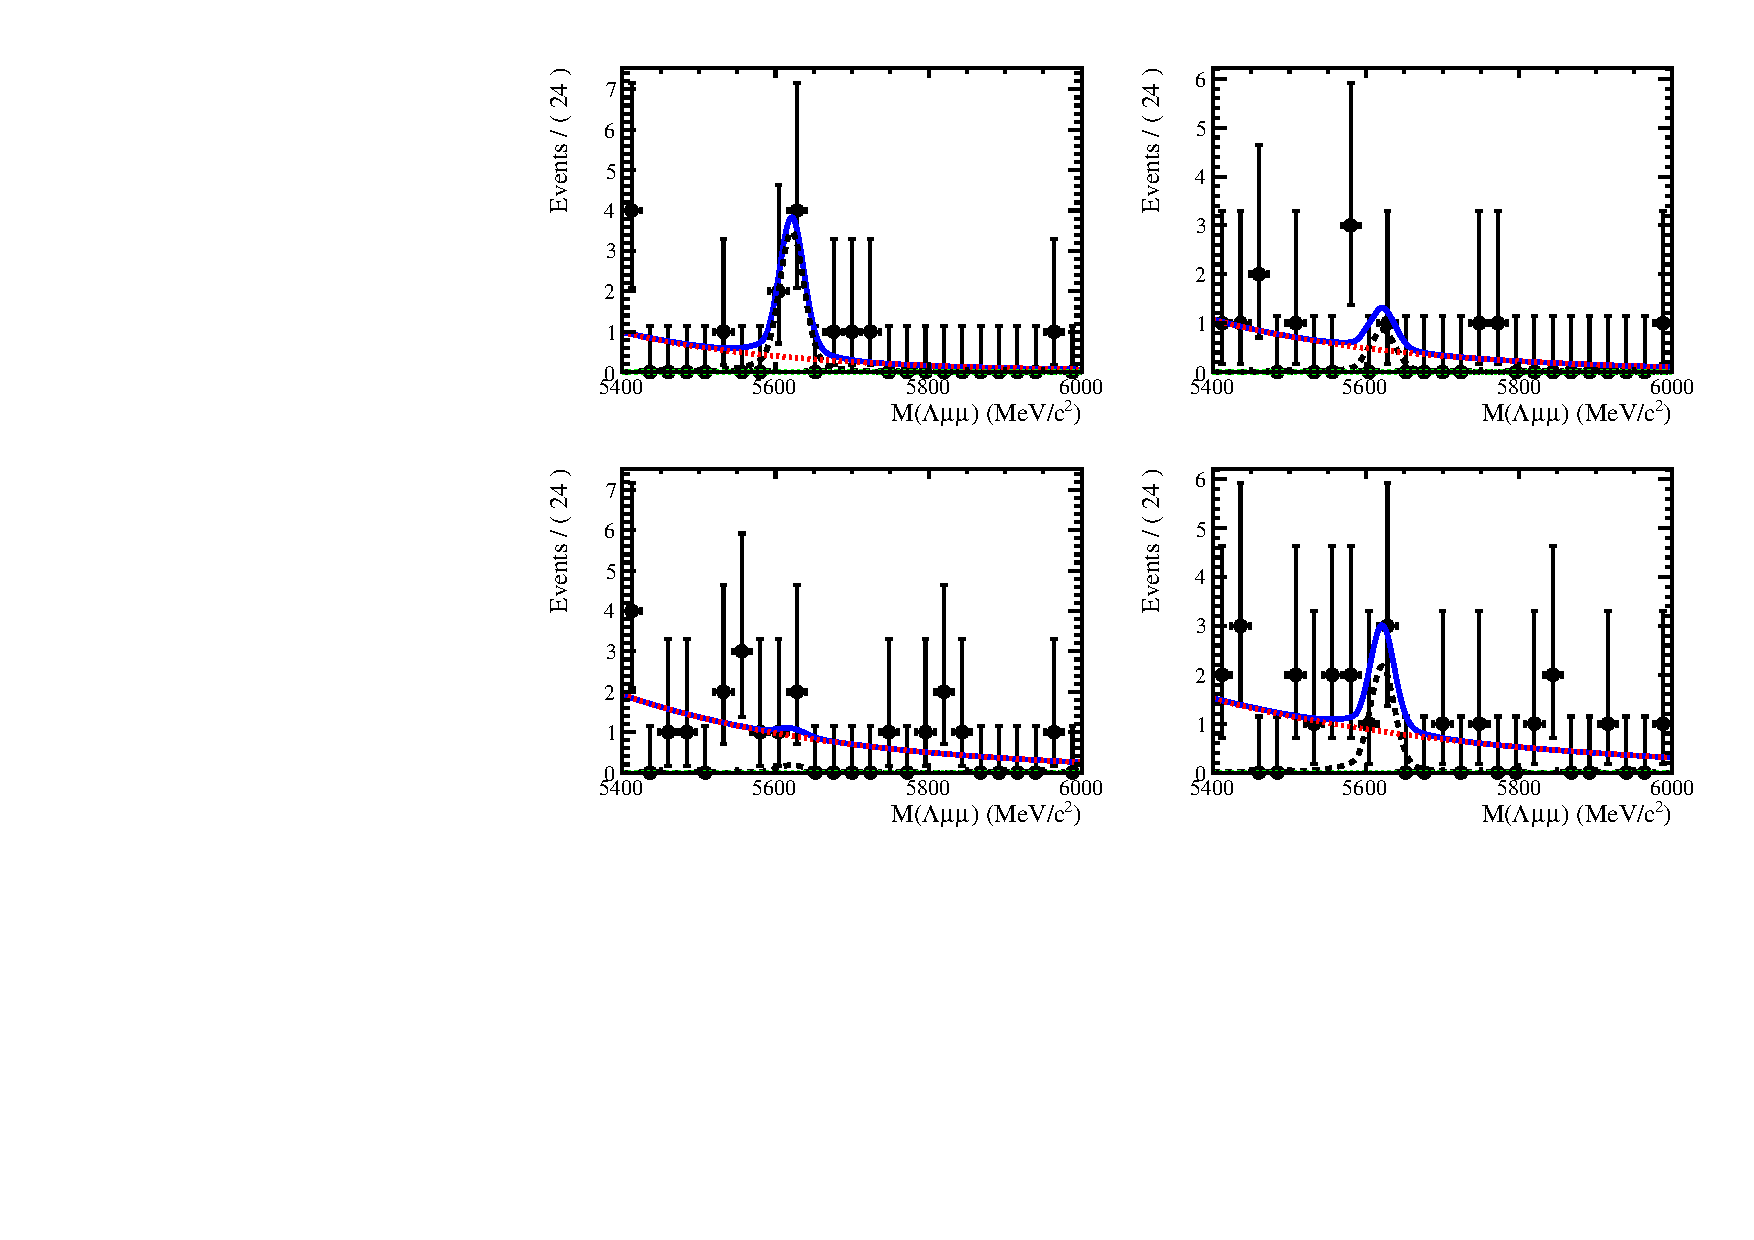
\includegraphics[width=1.\textwidth]{Lmumu/figs/MassFits/q2_fits_LL_plot2.pdf}
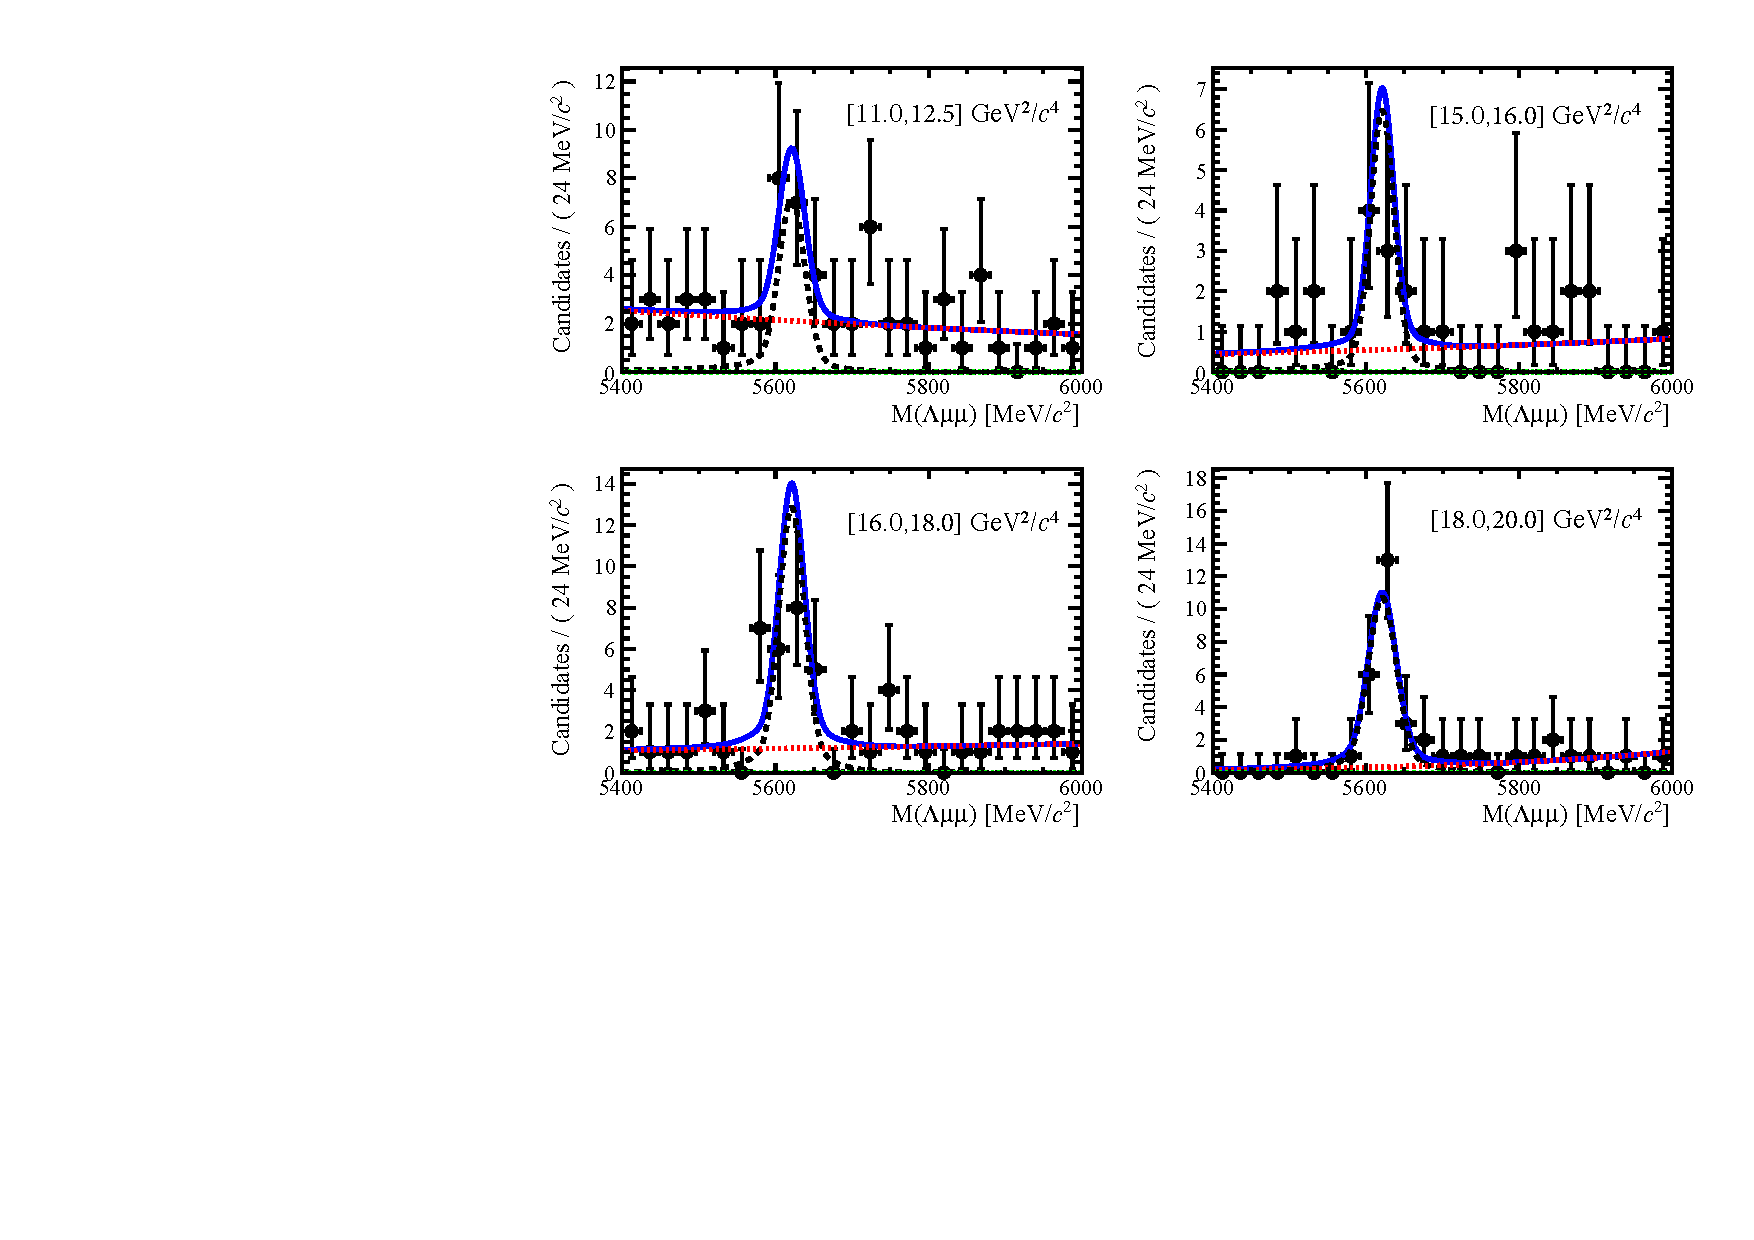
\includegraphics[width=1.\textwidth]{Lmumu/figs/MassFits/q2_fits_LL_plot1.pdf}
\caption{Invariant mass distributions of rare $\Lb\ra\Lz\mumu$ candidates in the considered \qsq bins
 %[0.1,2], [2,4], [4,6], [6,8], [11,12.5], [15,16], [16,18], [18,20]
 for long candidates. }
\label{fig:Lb_differentialFitLL}
\end{figure}



%\begin{table}
%\centering
%\caption{Values of exponential slope, $b$, and scale factors, $c$ found from the fit
%to the resonant data sample and fixed from the fit to the rare data sample.}
%\begin{tabular}{|c|c|c|}
%\hline
%Parameter  			 & Downstream & Long	\\ 
%\hline
%\multicolumn{3}{|c|}{ 15.0--20.0 \gevgevcccc}  \\
%\hline

%$b$ 				& $0.0006 \pm 0.0003$		 		& 	$0.0012 \pm 0.0008$        \\
%$c$ 				& $1.9027 \pm 0.0001$ 				&	$2.2910 \pm 0.0001$        \\
%%$N_{exp}$ 			& $393^{+23}_{-22}$	&	 $64^{+9}_{-8}$       \\

%\hline
%\multicolumn{3}{|c|}{ 1.1--6.0 \gevgevcccc}  \\

%\hline
%$b$ 				& $-0.0026 \pm 0.0004$				&	$-0.0036 \pm 0.0011$	 \\
%$c$ 				& $1.9208 \pm 0.0001$				&	$2.3504 \pm 0.0001$        \\
%%$N_{exp}$ 			& $203^{+15}_{-14}$	&	$34^{+7}_{-6}$       \\
%\hline

%\end{tabular}
%\label{tab:Lb_rareParam}
%\end{table}




\clearpage

